\chapter{Results and Interpretation}
\label{chap:SUSYresults}

Using the statistical framework outlined in the previous chapter, results are shown for the compatibility of the collected data with a \ac{SM}-only hypothesis in Section (\ref{sec:smhypothesis}). The data is further interpreted within the context of various \ac{SMS} models within Section (\ref{sec:resultsms}). 

\section{Compatibility with the Standard Model Hypothesis}
\label{sec:smhypothesis}

The \ac{SM} background only hypothesis is tested by removing any signal contributions within the signal and control samples, and the likelihood function defined in Equation (\ref{eq:totallikelihoodfunc}) maximised over all parameters using Rootfit \cite{2010acat.confE..57M} and MINUIT \cite{James:1975dr}. The results of the search consist of the observed yields in the hadronic signal sample, and the \mupjets, \dimupjets and \gpjets control samples. 

These observed yields along with the expectations and uncertainties given by the simultaneous fit for the hadronic signal region are given in Table \ref{tab:fitsdata}. The results obtained from the simultaneous fits, including that of the three control samples, are shown in Figure \ref{fig:result0blow}-\ref{fig:result4bhigh}, as summarised in Table \ref{tab:fitresults}. 

 \begin{table}[h!]
 \footnotesize
\begin{center}
\begin{tabular*}{0.55\textwidth}{@{\extracolsep{\fill}}cclc}
\hline
$n_{jet}$ & $n_{b}^{reco}$ & Control samples fitted & Figure  \\
\hline\hline
2-3 & 0 & \mupjets, \dimupjets, \gpjets & \ref{fig:result0blow} \\
2-3 & 1 & \mupjets, \dimupjets, \gpjets & \ref{fig:result1blow} \\
2-3 & 2 & \mupjets & \ref{fig:result2blow} \\
$\geq$4 & 0 & \mupjets, \dimupjets, \gpjets & \ref{fig:result0bhigh} \\
$\geq$4 & 1 & \mupjets, \dimupjets, \gpjets & \ref{fig:result1bhigh} \\
$\geq$4 & 2 & \mupjets & \ref{fig:result2bhigh} \\
$\geq$4 & 3 & \mupjets & \ref{fig:result3bhigh} \\
$\geq$4 & 4 & \mupjets & \ref{fig:result4bhigh} \\
\hline
\end{tabular*}
\end{center}
\caption[Summary of control samples used by each fit results, and the Figures in which they are displayed.]{Summary of control samples used by each fit results, and the Figures in which they are displayed.}\label{tab:fitresults}
\end{table}

 \begin{table}[h!]
 \footnotesize
\begin{center}
\begin{tabular*}{1.0\textwidth}{@{\extracolsep{\fill}}ccccccccccc}
\hline
& &&\multicolumn{8}{c}{\theht bin (\GeV)} \\
Cat & $n_{b}^{reco}$ & $n_{jet}$ &  275-325 & 325-375 & 375-475 & 474-575 & 575-675 & 675-775 & 775-875 & 875-$\infty$ \\
\hline\hline
SM & \multicolumn{1}{c}{\multirow{2}{*}{0}} & \multicolumn{1}{c}{\multirow{2}{*}{$\leq$ 3}} & 6235$^{+100}_{-67}$ & 2900$^{+60}_{-54}$ & $1955^{+34}_{-39}$& $558^{+14}_{-15}$ & $186^{+11}_{-10}$ & $51.3^{+3.4}_{-3.8}$ & $21.2^{+2.3}_{-2.2}$ & $16.1^{+1.7}_{-1.7}$ \\
Data &  &  & 6232 & 2904 & 1965 & 552 & 177 & 58 & 16 & 25 \\
\hline
SM & \multicolumn{1}{c}{\multirow{2}{*}{0}} & \multicolumn{1}{c}{\multirow{2}{*}{$\geq$ 4}} & 1010$^{+34}_{-24}$ & 447$^{+19}_{-16}$ & $390^{+19}_{-15}$& $250^{+12}_{-11}$ & $111^{+9}_{-7}$ & $53.3^{+4.3}_{-4.3}$ & $18.5^{+2.4}_{-2.4}$ & $19.4^{+2.5}_{-2.7}$ \\
Data &  &  & 1009 & 452 & 375 & 274 & 113 & 56 & 16 & 27 \\
\hline
SM & \multicolumn{1}{c}{\multirow{2}{*}{1}} & \multicolumn{1}{c}{\multirow{2}{*}{$\leq$ 3}} & 1162$^{+37}_{-29}$ & 481$^{+18}_{-19}$ & $341^{+15}_{-16}$& $86.7^{+4.2}_{-5.6}$ & $24.8^{+2.8}_{-2.7}$ & $7.2^{+1.1}_{-1.0}$ & $3.3^{+0.7}_{-0.7}$ & $2.1^{+0.5}_{-0.5}$ \\
Data &  &  & 1164 & 473 & 329 & 95 & 23 & 8 & 4 & 1 \\
\hline
SM & \multicolumn{1}{c}{\multirow{2}{*}{1}} & \multicolumn{1}{c}{\multirow{2}{*}{$\geq$ 4}} & 521$^{+25}_{-17}$ & 232$^{+15}_{-12}$ & $188^{+12}_{-11}$& $106^{+6}_{-6}$ & $42.1^{+4.1}_{-4.4}$ & $17.9^{+2.2}_{-2.0}$ & $9.8^{+1.5}_{-1.4}$ & $6.8^{+1.2}_{-1.1}$ \\
Data &  &  & 515 & 236 & 204 & 92 & 51 & 13 & 13 & 6 \\
\hline
SM & \multicolumn{1}{c}{\multirow{2}{*}{2}} & \multicolumn{1}{c}{\multirow{2}{*}{$\leq$ 3}} & 224$^{+15}_{-14}$ & 98.2$^{+8.4}_{-6.4}$ & $59.0^{+5.2}_{-6.0}$& $12.8^{+1.6}_{-1.6}$ & $3.0^{+0.9}_{-0.7}$ & $0.5^{+0.2}_{-0.2}$ & $0.1^{+0.1}_{-0.1}$ & $0.1^{+0.1}_{-0.1}$ \\
Data &  &  & 222 & 107 & 58 & 12 & 5 & 1 & 0 & 0 \\
\hline
SM & \multicolumn{1}{c}{\multirow{2}{*}{2}} & \multicolumn{1}{c}{\multirow{2}{*}{$\geq$ 4}} & 208$^{+17}_{-9}$ & 103$^{+9}_{-7}$ & $85.9^{+7.2}_{-6.9}$& $51.7^{+4.6}_{-4.7}$ & $19.9^{+3.4}_{-3.0}$ & $6.8^{+1.2}_{-1.3}$ & $1.7^{+0.7}_{-0.4}$ & $1.3^{+0.4}_{-0.3}$ \\
Data &  &  & 204 & 107 & 84 & 59 & 24 & 5 & 1 & 2 \\
\hline
SM & \multicolumn{1}{c}{\multirow{2}{*}{3}} & \multicolumn{1}{c}{\multirow{2}{*}{$\geq$ 4}} & 25.3$^{+5.0}_{-4.2}$ & 11.7$^{+1.7}_{-1.8}$ & $6.7^{+1.4}_{-1.2}$& $3.9^{+0.8}_{-0.8}$ & $2.3^{+0.6}_{-0.6}$ & $1.2^{+0.3}_{-0.4}$ & $0.3^{+0.2}_{-0.1}$ & $0.1^{+0.1}_{-0.1}$ \\
Data &  &  & 25 & 13 & 4 & 2 & 2 & 3 & 0 & 0 \\
\hline
SM & \multicolumn{1}{c}{\multirow{2}{*}{4}} & \multicolumn{1}{c}{\multirow{2}{*}{$\geq$ 4}} & 0.9$^{+0.4}_{-0.7}$ & 0.3$^{+0.2}_{-0.2}$ & \multicolumn{6}{c}{$0.6^{+0.3}_{-0.3}$} \\
Data &  &  & 1 & 0 & \multicolumn{6}{c}{2} \\
\hline
\end{tabular*}
\end{center}
\caption[Comparison of the measured yields in each \theht, $n_{jet}$ and $n_{b}^{reco}$ jet multiplicity bins for the hadronic sample with the \ac{SM} expectations and combined statistical and systematic uncertainties given by the simultaneous fit.]{Comparison of the measured yields in each \theht, $n_{jet}$ and $n_{b}^{reco}$ jet multiplicity bins for the hadronic sample with the \ac{SM} expectations and combined statistical and systematic uncertainties given by the simultaneous fit.}\label{tab:fitsdata}
\end{table}

The figures show a comparison between the observed yields and the \ac{SM} expectations across all \theht bins, and in all $n_{jet}$ and $n_{b}^{reco}$ multiplicity categories. In all categories the samples are well described by the \ac{SM} only hypothesis. In particular no significant excess is observed above \ac{SM} expectation within the hadronic signal region. 

Given the lack of an excess in data hinting at a possible supersymmetric signature within the data, interpretations are made on the production masses and cross-section of a range of \ac{SUSY} decay topologies within the following section.

\begin{figure}[ht]
\footnotesize
\centering
\begin{minipage}[b]{0.48 \linewidth}
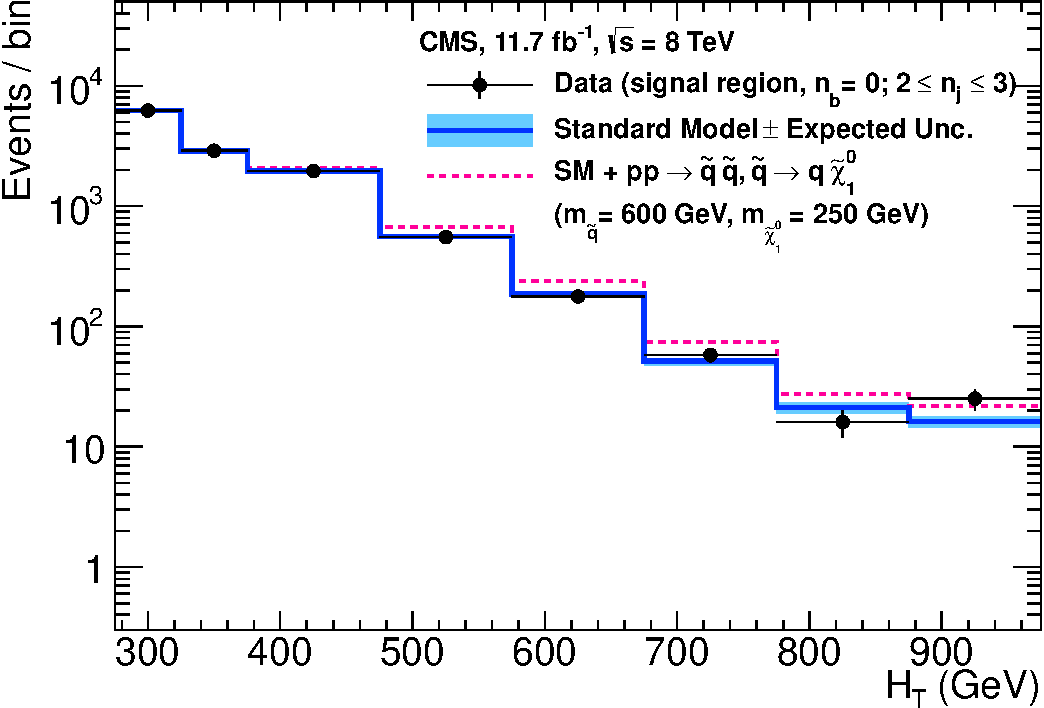
\includegraphics[width = 1.0\linewidth]{plots/hadronic_0b_le3j_logy.pdf}
\centering (a)  Hadronic sample, $2 \leq n_{jet} \leq 3$ and $n_{b}^{reco} = 0$ 
\end{minipage}
\quad
\begin{minipage}[b]{0.48\linewidth}
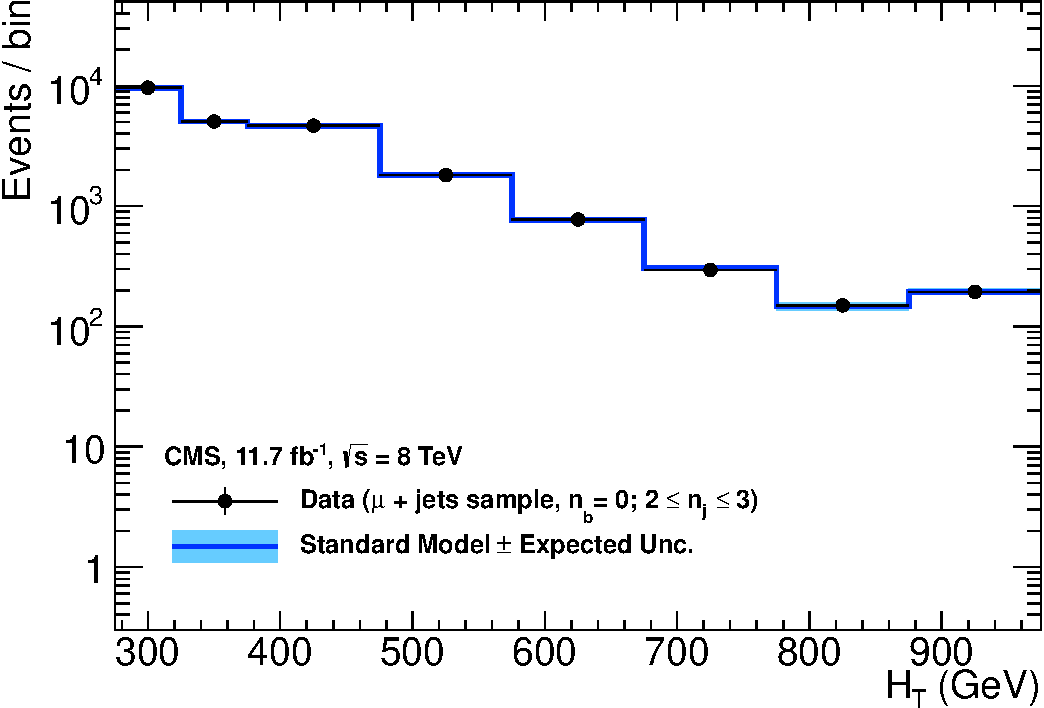
\includegraphics[width = 1.0\linewidth]{plots/muon_0b_le3j_logy.pdf}
\centering (b)  \mupjets sample, $2 \leq n_{jet} \leq 3$ and $n_{b}^{reco} = 0$  
\end{minipage} \\
\vspace{0.4cm}
\begin{minipage}[b]{0.48 \linewidth}
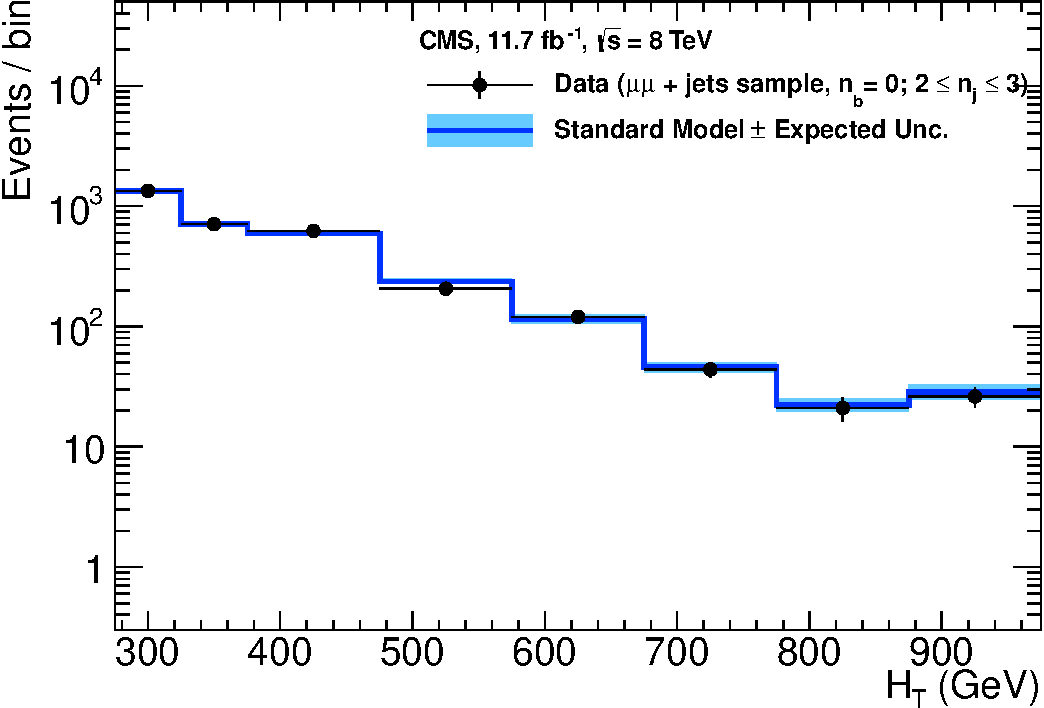
\includegraphics[width = 1.0\linewidth]{plots/mumu_0b_le3j_logy.pdf}
\centering (c$)$ \dimupjets sample, $2 \leq n_{jet} \leq 3$ and $n_{b}^{reco} = 0$ 
\end{minipage}
\quad
\begin{minipage}[b]{0.48\linewidth}
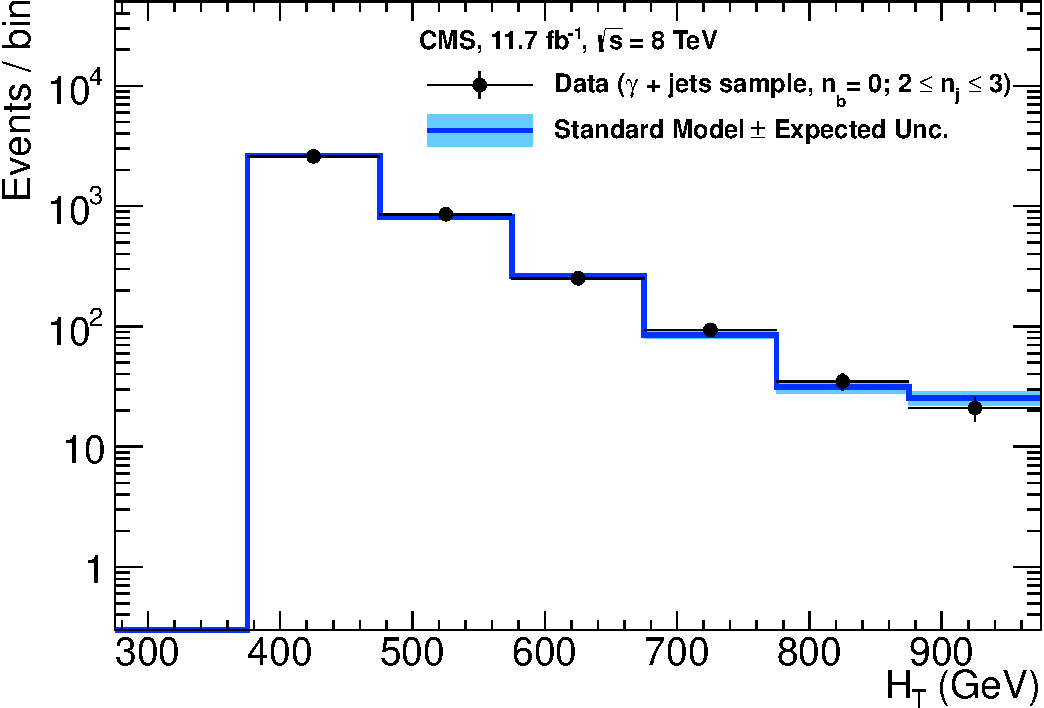
\includegraphics[width = 1.0\linewidth]{plots/photon_0b_le3j_logy.pdf}
\centering (d)  \gpjets sample, $2 \leq n_{jet} \leq 3$ and $n_{b}^{reco} = 0$ 
\end{minipage}
\caption[Comparison of the observed yields and \ac{SM} expectations given by the simultaneous fit in bins of \theht for the (a) hadronic, (b) \mupjets, (c$)$ \dimupjets and (d) \gpjets samples when requiring $n_{b}^{reco}$ = 0 and $n_{jet} \leq 3$.]{Comparison of the observed yields and \ac{SM} expectations given by the simultaneous fit in bins of \theht for the (a) hadronic, (b) \mupjets, (c$)$ \dimupjets and (d) \gpjets samples when requiring $n_{b}^{reco}$ = 0 and $n_{jet} \leq 3$. The observed event yields in data (black dots) and the expectations and their uncertainties for all SM processes (blue line with light blue bands) are shown. An example signal expectation (red solid line) for the $D1$ \ac{SMS} signal point from Table \ref{tab:sms_model_table} is superimposed on the \ac{SM} background expectation.}
\label{fig:result0blow}
\end{figure}

\begin{figure}[ht]
\footnotesize
\centering
\begin{minipage}[b]{0.48 \linewidth}
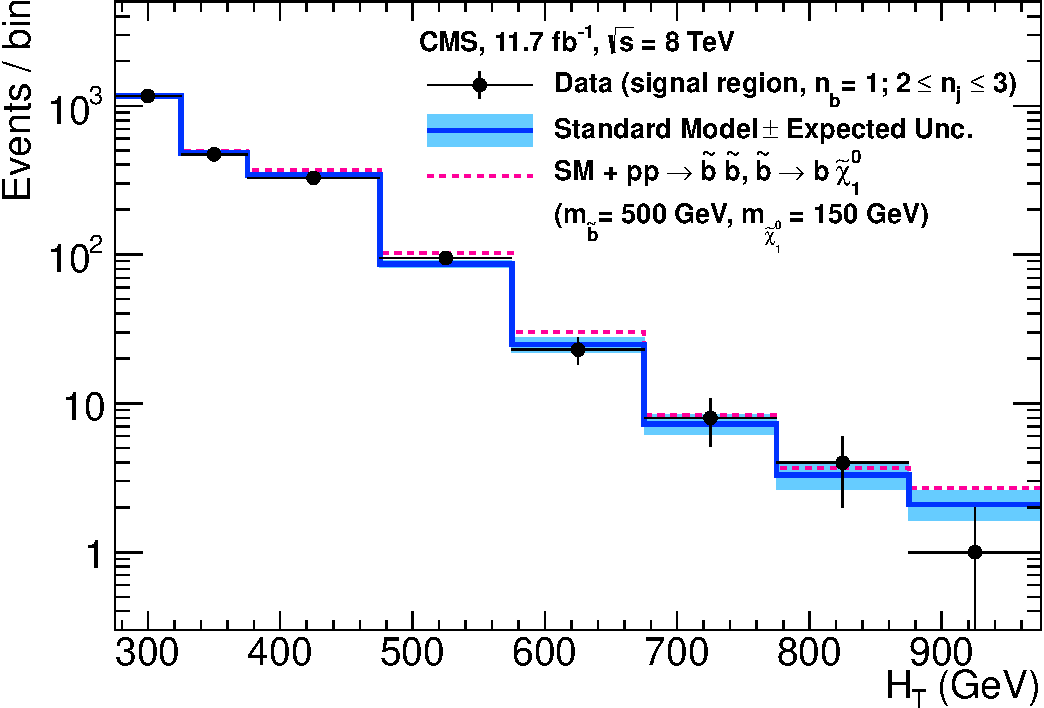
\includegraphics[width = 1.0\linewidth]{plots/hadronic_1b_le3j_logy.pdf}
\centering (a)  Hadronic sample, $2 \leq n_{jet} \leq 3$ and $n_{b}^{reco} = 1$ 
\end{minipage}
\quad
\begin{minipage}[b]{0.48\linewidth}
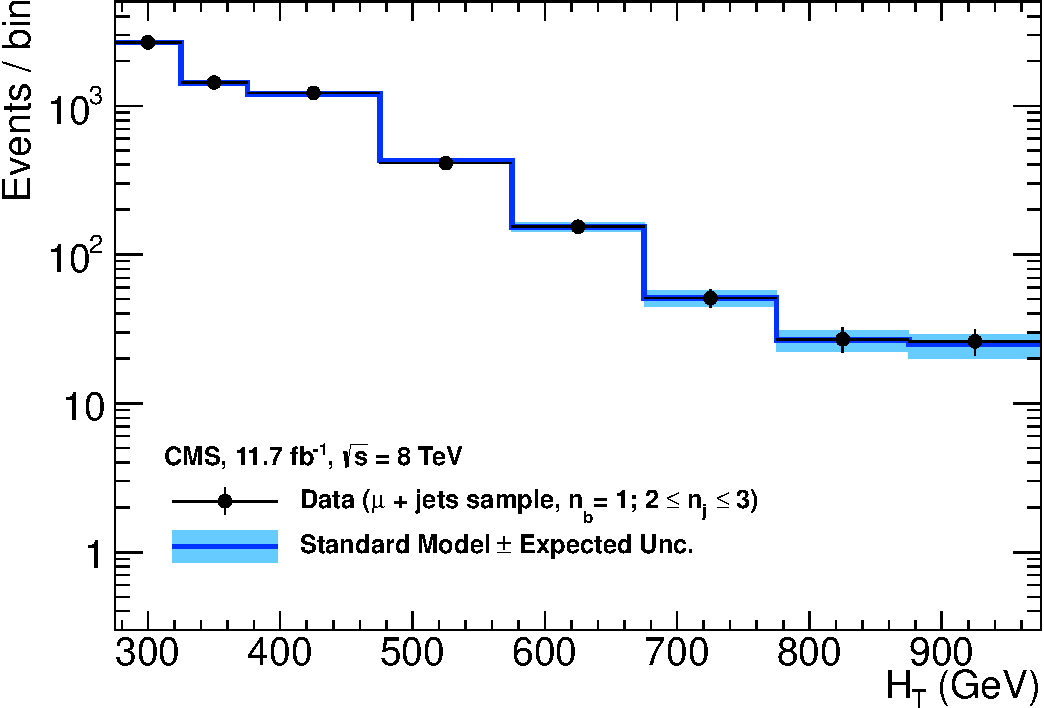
\includegraphics[width = 1.0\linewidth]{plots/muon_1b_le3j_logy.pdf}
\centering (b)  \mupjets sample, $2 \leq n_{jet} \leq 3$ and $n_{b}^{reco} = 1$  
\end{minipage} \\
\vspace{0.4cm}
\begin{minipage}[b]{0.48 \linewidth}
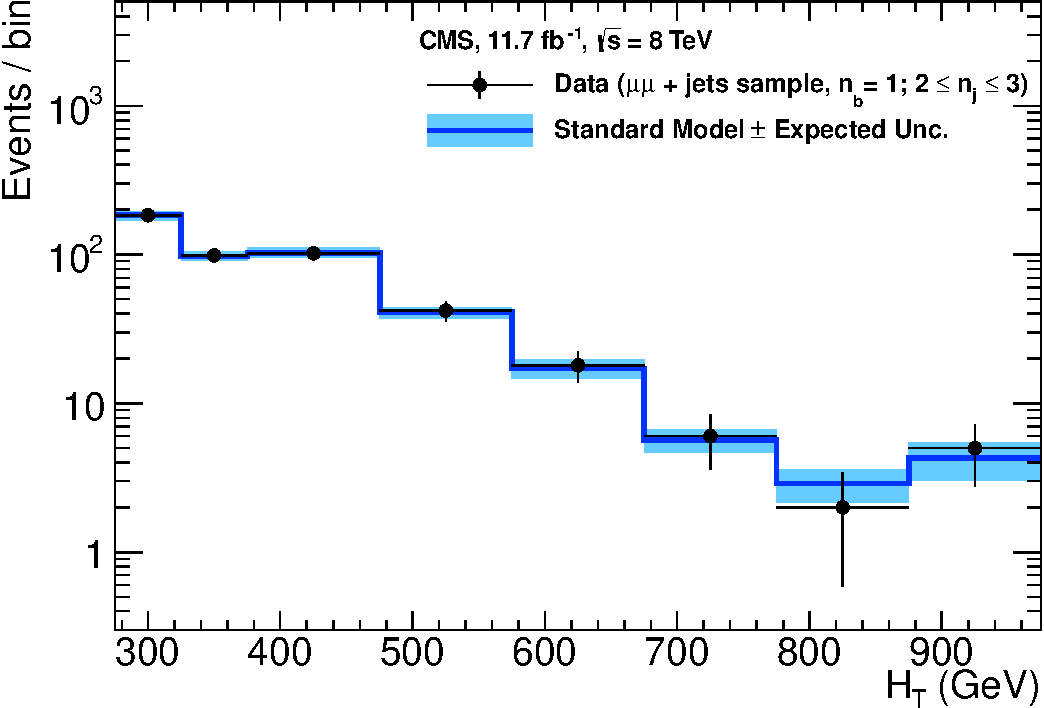
\includegraphics[width = 1.0\linewidth]{plots/mumu_1b_le3j_logy.pdf}
\centering (c$)$ \dimupjets sample, $2 \leq n_{jet} \leq 3$ and $n_{b}^{reco} = 1$ 
\end{minipage}
\quad
\begin{minipage}[b]{0.48\linewidth}
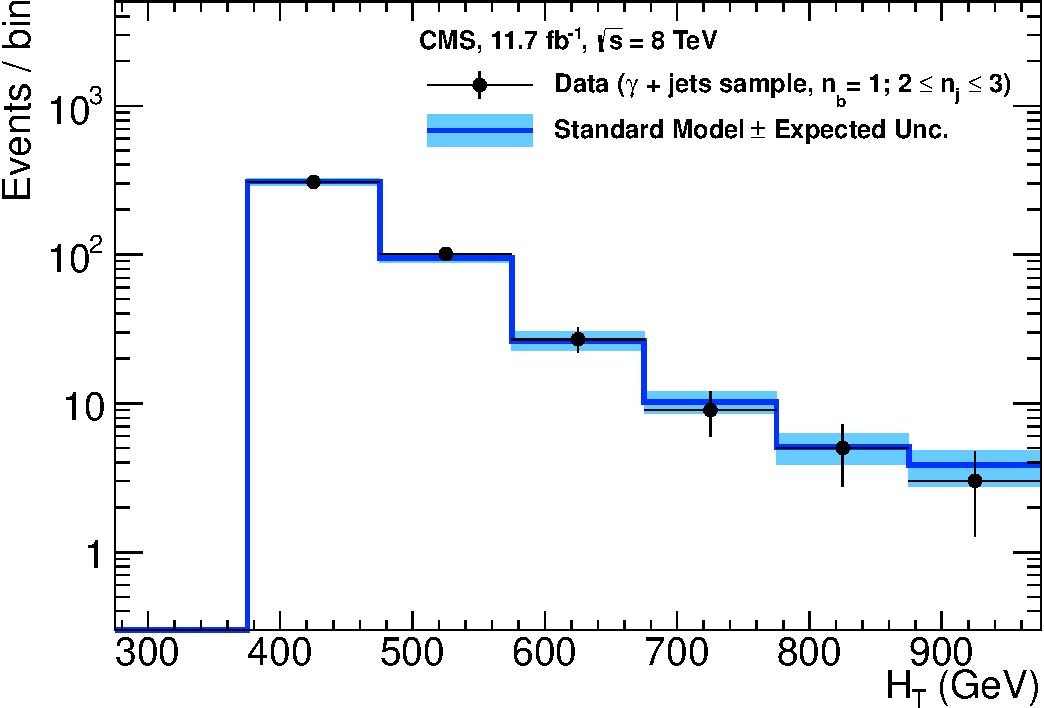
\includegraphics[width = 1.0\linewidth]{plots/photon_1b_le3j_logy.pdf}
\centering (d)  \gpjets sample, $2 \leq n_{jet} \leq 3$ and $n_{b}^{reco} = 1$ 
\end{minipage}
\caption[Comparison of the observed yields and \ac{SM} expectations given by the simultaneous fit in bins of \theht for the (a) hadronic, (b) \mupjets, (c$)$ \dimupjets and (d) \gpjets samples when requiring $n_{b}^{reco}$ = 1 and $n_{jet} \leq 3$.]{Comparison of the observed yields and \ac{SM} expectations given by the simultaneous fit in bins of \theht for the (a) hadronic, (b) \mupjets, (c$)$ \dimupjets and (d) \gpjets samples when requiring $n_{b}^{reco}$ = 1 and $n_{jet} \leq 3$. The observed event yields in data (black dots) and the expectations and their uncertainties for all SM processes (blue line with light blue bands) are shown. An example signal expectation (red solid line) for the $D2$ \ac{SMS} signal point from Table \ref{tab:sms_model_table} is superimposed on the \ac{SM} background expectation.}
\label{fig:result1blow}
\end{figure}

\begin{figure}[ht]
\footnotesize
\centering
\begin{minipage}[b]{0.48 \linewidth}
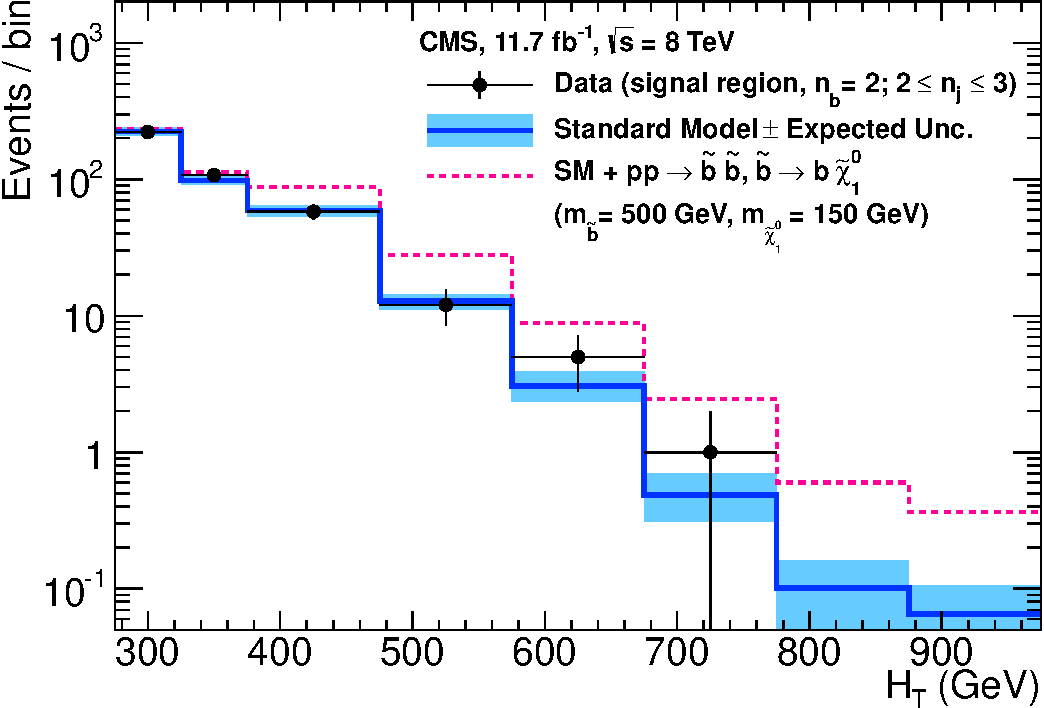
\includegraphics[width = 1.0\linewidth]{plots/hadronic_2b_le3j_logy.pdf}
\centering (a)  Hadronic sample, $2 \leq n_{jet} \leq 3$ and $n_{b}^{reco} = 2$ 
\end{minipage}
\quad
\begin{minipage}[b]{0.48\linewidth}
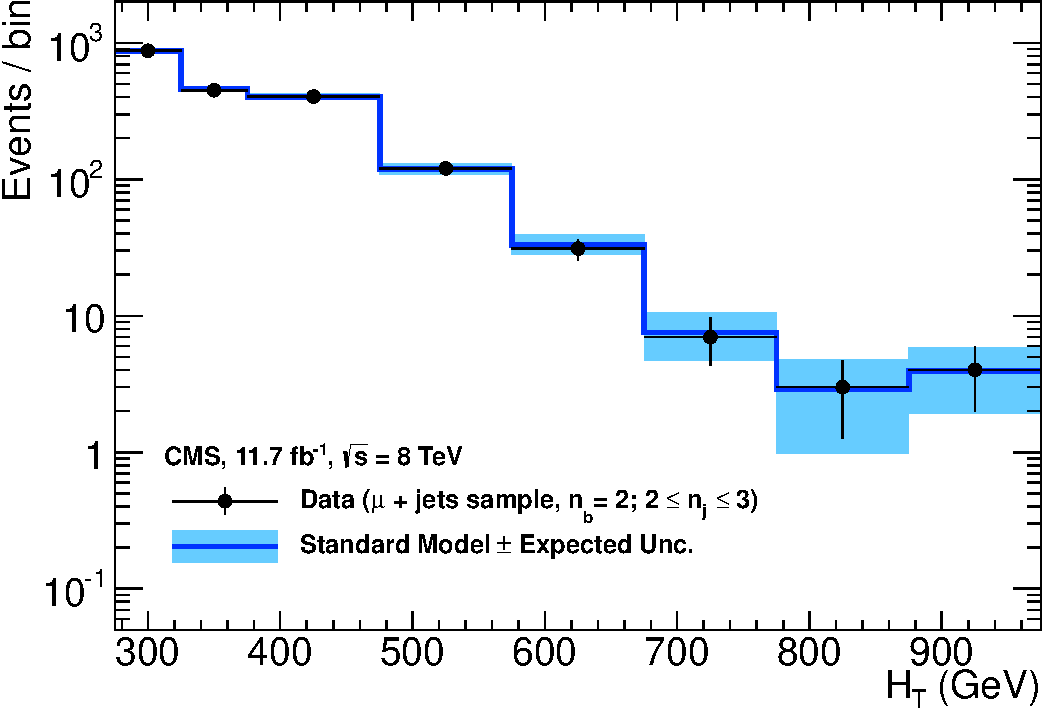
\includegraphics[width = 1.0\linewidth]{plots/muon_2b_le3j_logy.pdf}
\centering (b)  \mupjets sample, $2 \leq n_{jet} \leq 3$ and $n_{b}^{reco} = 2$  
\end{minipage} \\
\caption[Comparison of the observed yields and \ac{SM} expectations given by the simultaneous fit in bins of \theht for the (a) hadronic, (b) \mupjets, (c$)$ \dimupjets and (d) \gpjets samples when requiring $n_{b}^{reco}$ = 2 and $n_{jet} \leq 3$.]{Comparison of the observed yields and \ac{SM} expectations given by the simultaneous fit in bins of \theht for the (a) hadronic, (b) \mupjets, (c$)$ \dimupjets and (d) \gpjets samples when requiring $n_{b}^{reco}$ = 2 and $n_{jet} \leq 3$. The observed event yields in data (black dots) and the expectations and their uncertainties for all SM processes (blue line with light blue bands) are shown. An example signal expectation (red solid line) for the $D2$ \ac{SMS} signal point from Table \ref{tab:sms_model_table} is superimposed on the \ac{SM} background expectation.}
\label{fig:result2blow}
\end{figure}

\begin{figure}[ht]
\footnotesize
\centering
\begin{minipage}[b]{0.48 \linewidth}
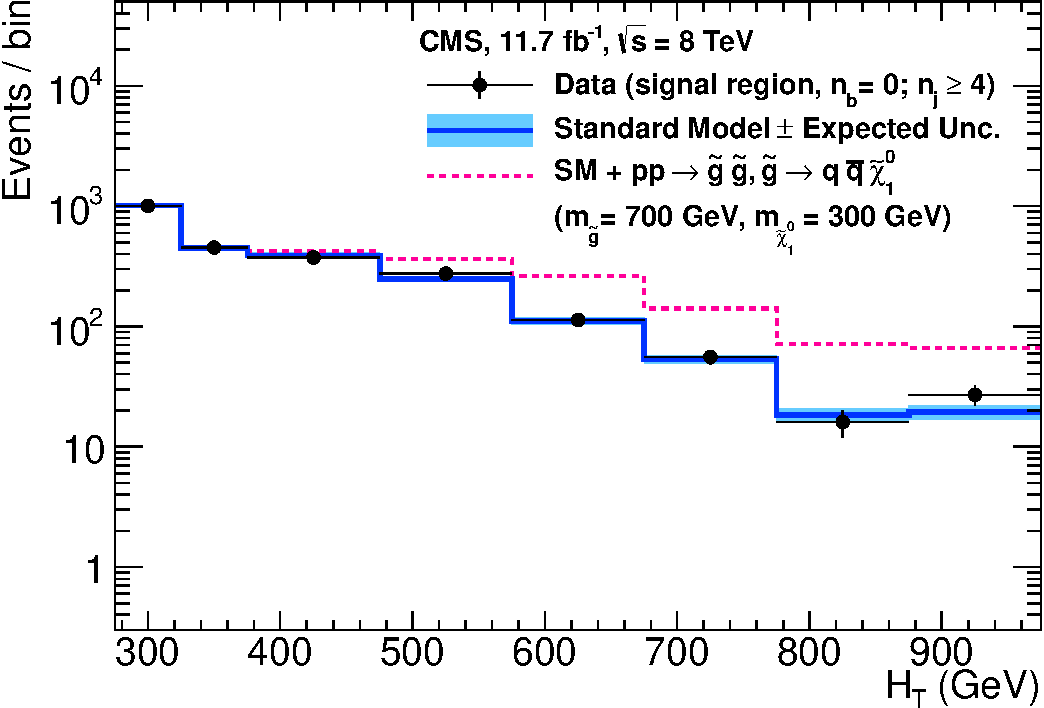
\includegraphics[width = 1.0\linewidth]{plots/hadronic_0b_ge4j_logy.pdf}
\centering (a)  Hadronic sample, $n_{jet} \geq 4$ and $n_{b}^{reco} = 0$ 
\end{minipage}
\quad
\begin{minipage}[b]{0.48\linewidth}
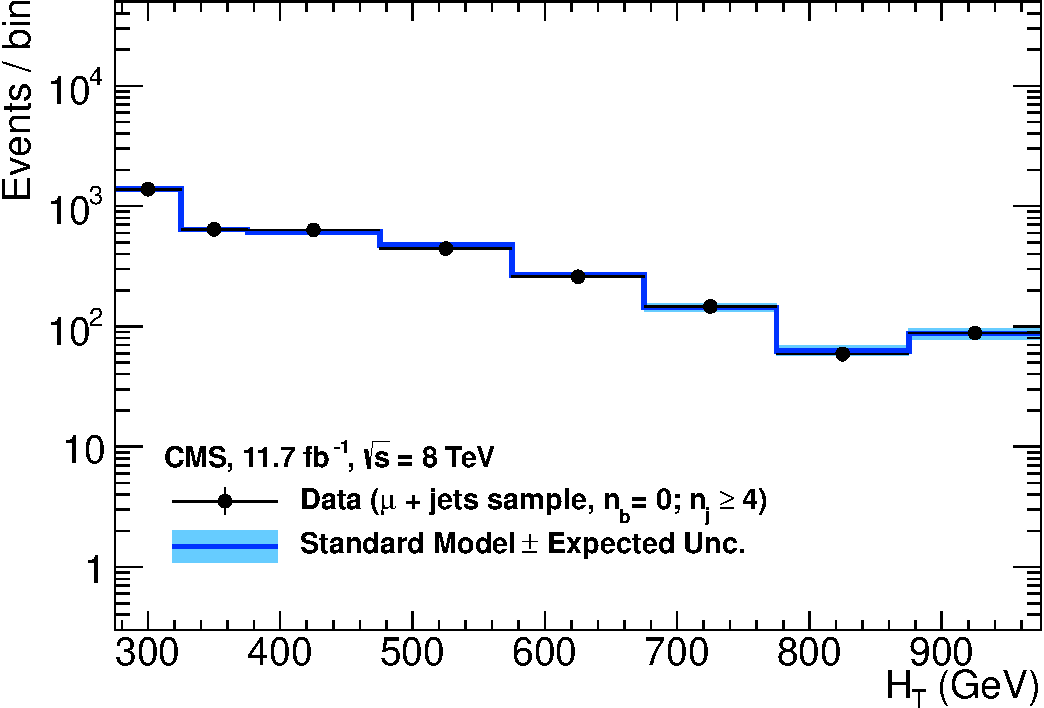
\includegraphics[width = 1.0\linewidth]{plots/muon_0b_ge4j_logy.pdf}
\centering (b)  \mupjets sample, $n_{jet} \geq 4$ and $n_{b}^{reco} = 0$  
\end{minipage} \\
\vspace{0.4cm}
\begin{minipage}[b]{0.48 \linewidth}
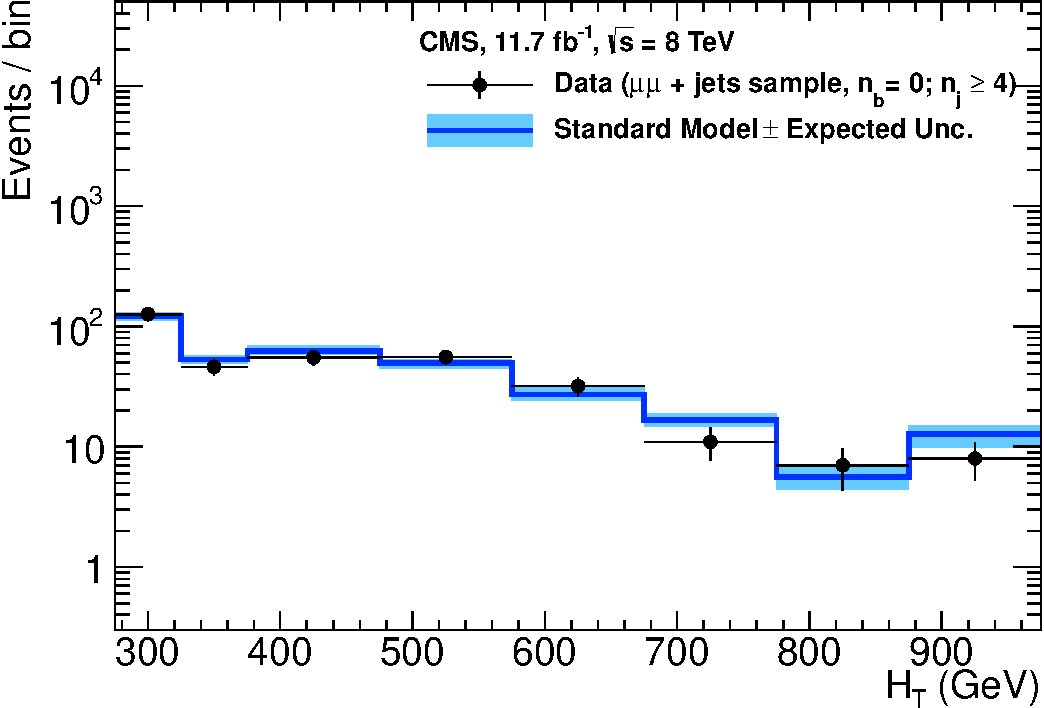
\includegraphics[width = 1.0\linewidth]{plots/mumu_0b_ge4j_logy.pdf}
\centering (c$)$ \dimupjets sample, $n_{jet} \geq 4$ and $n_{b}^{reco} = 0$ 
\end{minipage}
\quad
\begin{minipage}[b]{0.48\linewidth}
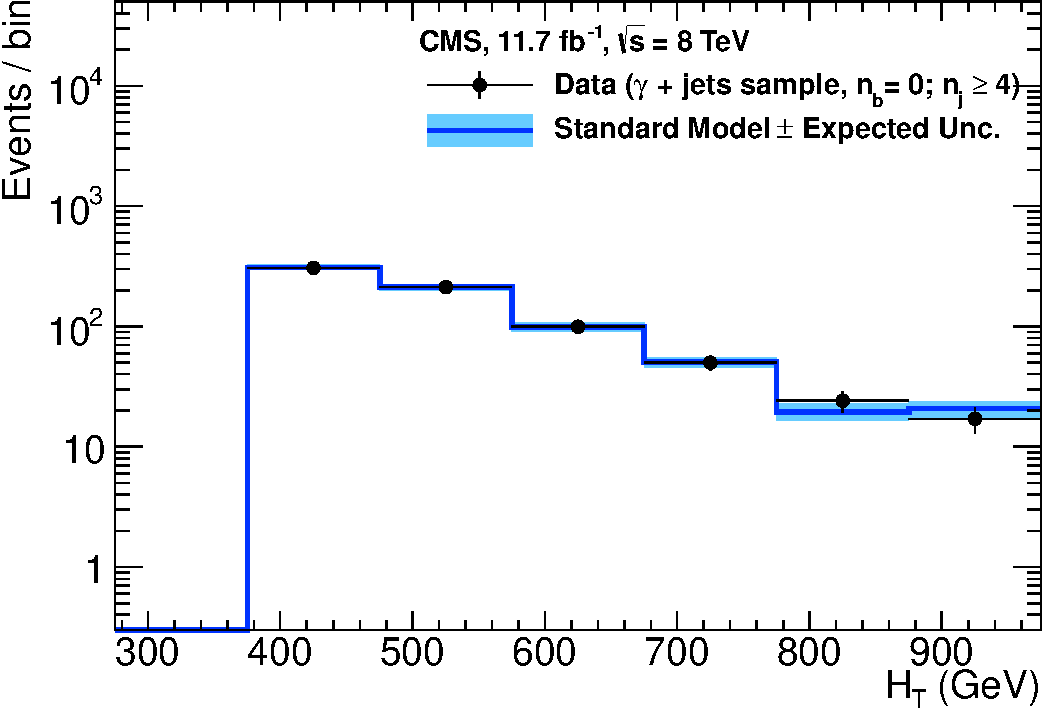
\includegraphics[width = 1.0\linewidth]{plots/photon_0b_ge4j_logy.pdf}
\centering (d)  \gpjets sample, $n_{jet} \geq 4$ and $n_{b}^{reco} = 0$ 
\end{minipage}
\caption[Comparison of the observed yields and \ac{SM} expectations given by the simultaneous fit in bins of \theht for the (a) hadronic, (b) \mupjets, (c$)$ \dimupjets and (d) \gpjets samples when requiring $n_{b}^{reco}$ = 0 and $n_{jet} \geq 4$.]{Comparison of the observed yields and \ac{SM} expectations given by the simultaneous fit in bins of \theht for the (a) hadronic, (b) \mupjets, (c$)$ \dimupjets and (d) \gpjets samples when requiring $n_{b}^{reco}$ = 0 and $n_{jet} \geq 4$. The observed event yields in data (black dots) and the expectations and their uncertainties for all SM processes (blue line with light blue bands) are shown. An example signal expectation (red solid line) for the $D2$ \ac{SMS} signal point from Table \ref{tab:sms_model_table} is superimposed on the \ac{SM} background expectation.}
\label{fig:result0bhigh}
\end{figure}


\begin{figure}[ht]
\footnotesize
\centering
\begin{minipage}[b]{0.48 \linewidth}
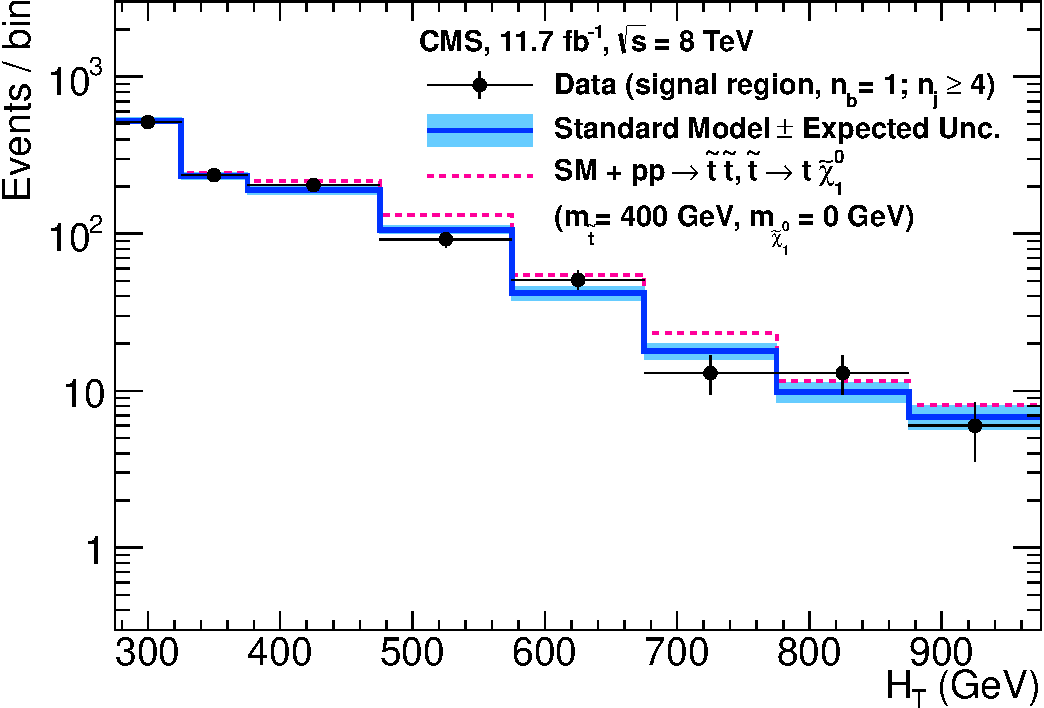
\includegraphics[width = 1.0\linewidth]{plots/hadronic_1b_ge4j_logy.pdf}
\centering (a)  Hadronic sample, $n_{jet} \geq 4$ and $n_{b}^{reco} = 1$ 
\end{minipage}
\quad
\begin{minipage}[b]{0.48\linewidth}
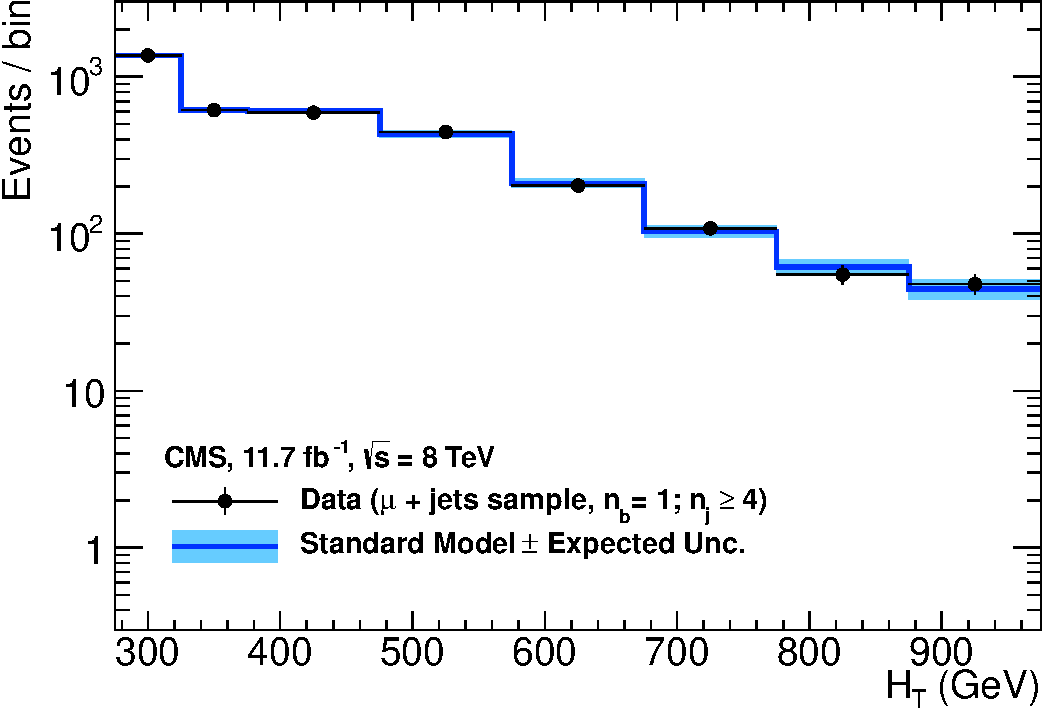
\includegraphics[width = 1.0\linewidth]{plots/muon_1b_ge4j_logy.pdf}
\centering (b)  \mupjets sample, $n_{jet} \geq 4$ and $n_{b}^{reco} = 1$  
\end{minipage} \\
\vspace{0.4cm}
\begin{minipage}[b]{0.48 \linewidth}
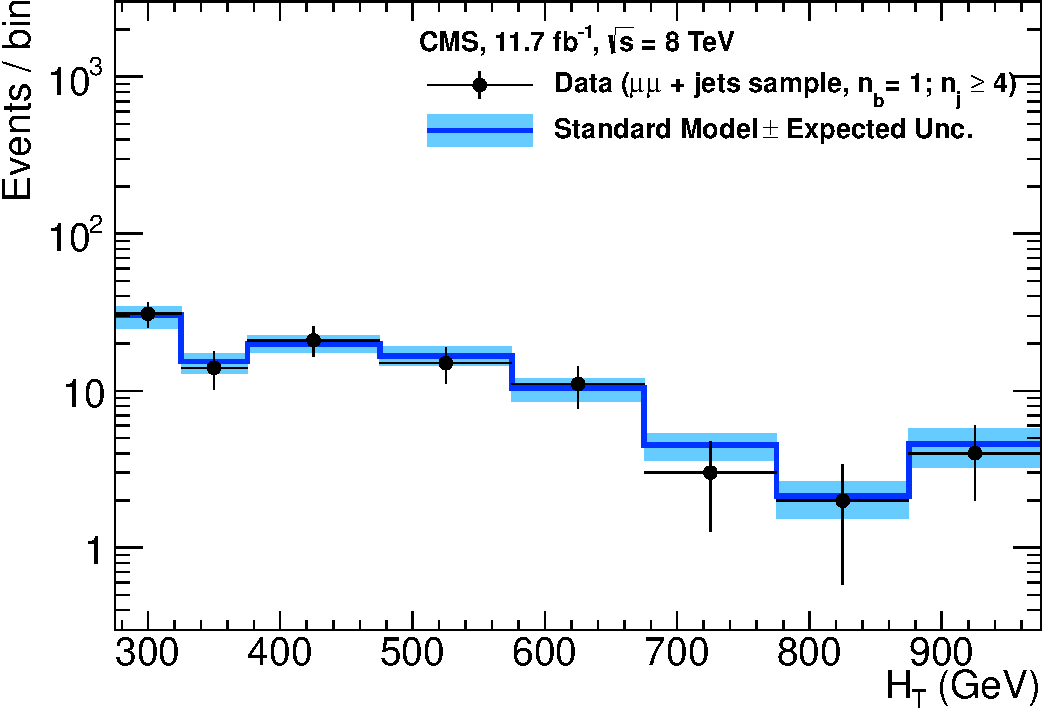
\includegraphics[width = 1.0\linewidth]{plots/mumu_1b_ge4j_logy.pdf}
\centering (c$)$ \dimupjets sample, $n_{jet} \geq 4$ and $n_{b}^{reco} = 1$ 
\end{minipage}
\quad
\begin{minipage}[b]{0.48\linewidth}
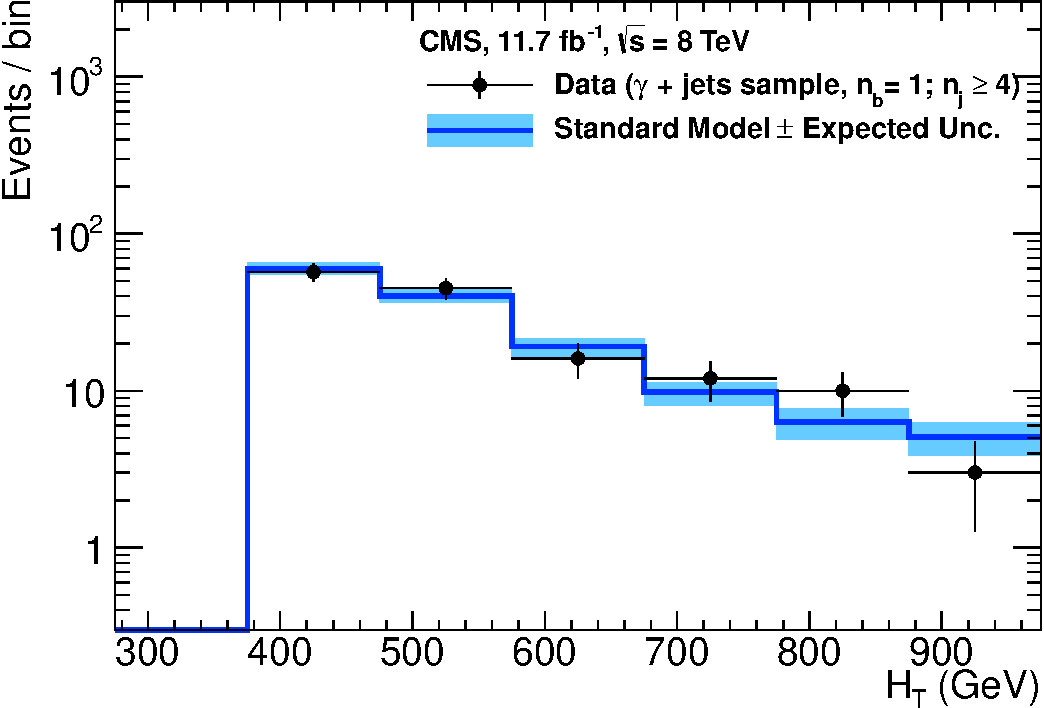
\includegraphics[width = 1.0\linewidth]{plots/photon_1b_ge4j_logy.pdf}
\centering (d)  \gpjets sample, $n_{jet} \geq 4$ and $n_{b}^{reco} = 1$ 
\end{minipage}
\caption[Comparison of the observed yields and \ac{SM} expectations given by the simultaneous fit in bins of \theht for the (a) hadronic, (b) \mupjets, (c$)$ \dimupjets and (d) \gpjets samples when requiring $n_{b}^{reco}$ = 1 and $n_{jet} \geq 4$.]{Comparison of the observed yields and \ac{SM} expectations given by the simultaneous fit in bins of \theht for the (a) hadronic, (b) \mupjets, (c$)$ \dimupjets and (d) \gpjets samples when requiring $n_{b}^{reco}$ = 1 and $n_{jet} \geq 4$. The observed event yields in data (black dots) and the expectations and their uncertainties for all SM processes (blue line with light blue bands) are shown.}
\label{fig:result1bhigh}
\end{figure}

\begin{figure}[ht]
\footnotesize
\centering
\begin{minipage}[b]{0.48 \linewidth}
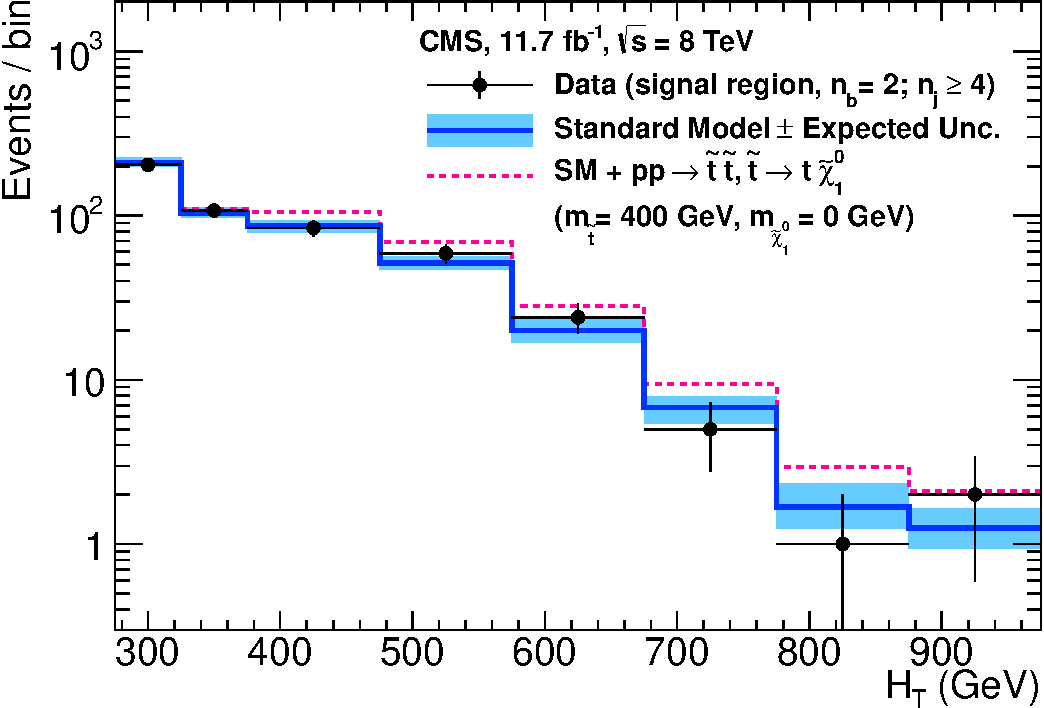
\includegraphics[width = 1.0\linewidth]{plots/hadronic_2b_ge4j_logy.pdf}
\centering (a)  Hadronic sample, $n_{jet} \geq 4$ and $n_{b}^{reco} = 2$ 
\end{minipage}
\quad
\begin{minipage}[b]{0.48\linewidth}
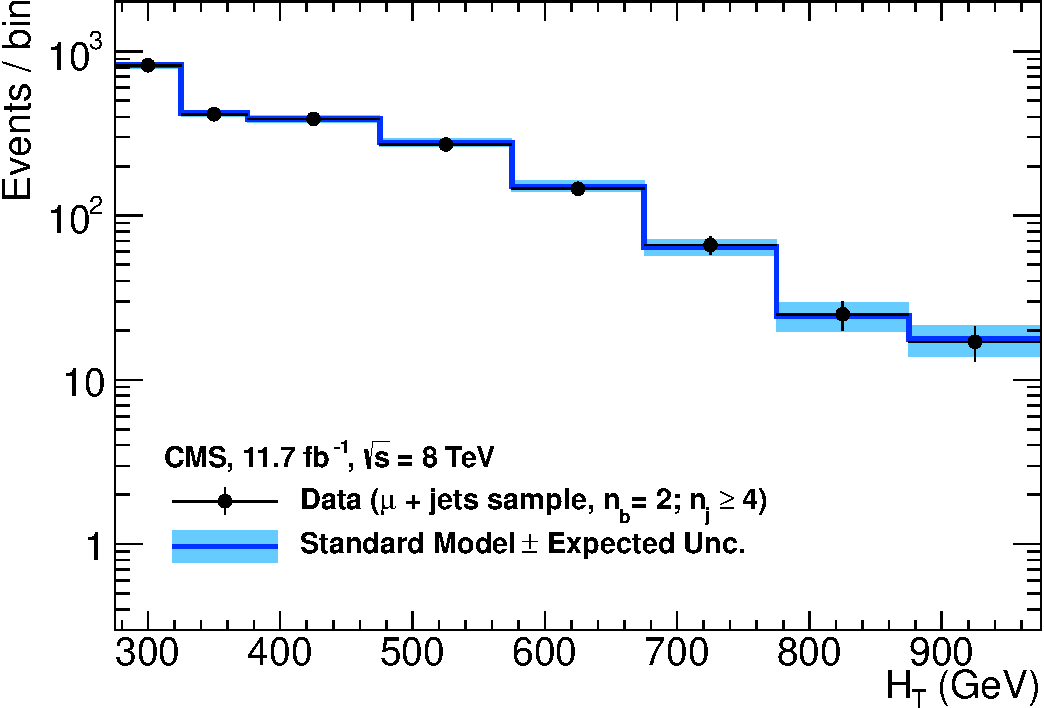
\includegraphics[width = 1.0\linewidth]{plots/muon_2b_ge4j_logy.pdf}
\centering (b)  \mupjets sample, $n_{jet} \geq 4$ and $n_{b}^{reco} = 2$  
\end{minipage} \\
\caption[Comparison of the observed yields and \ac{SM} expectations given by the simultaneous fit in bins of \theht for the (a) hadronic, (b) \mupjets, (c$)$ \dimupjets and (d) \gpjets samples when requiring $n_{b}^{reco}$ = 2 and $n_{jet} \geq 4$.]{Comparison of the observed yields and \ac{SM} expectations given by the simultaneous fit in bins of \theht for the (a) hadronic, (b) \mupjets, (c$)$ \dimupjets and (d) \gpjets samples when requiring $n_{b}^{reco}$ = 2 and $n_{jet} \geq 4$. The observed event yields in data (black dots) and the expectations and their uncertainties for all SM processes (blue line with light blue bands) are shown. An example signal expectation (red solid line) for the $D3$ \ac{SMS} signal point from Table \ref{tab:sms_model_table} is superimposed on the \ac{SM} background expectation.}
\label{fig:result2bhigh}
\end{figure}

\begin{figure}[ht]
\footnotesize
\centering
\begin{minipage}[b]{0.48 \linewidth}
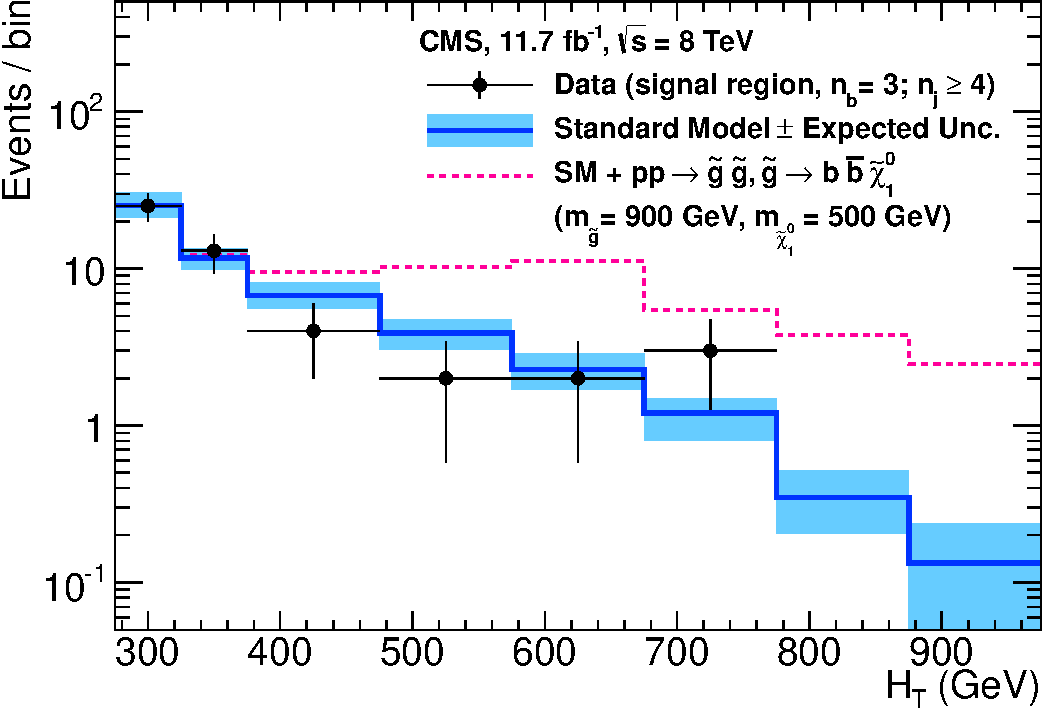
\includegraphics[width = 1.0\linewidth]{plots/hadronic_3b_ge4j_logy.pdf}
\centering (a)  Hadronic sample, $n_{jet} \geq 4$ and $n_{b}^{reco} = 3$ 
\end{minipage}
\quad
\begin{minipage}[b]{0.48\linewidth}
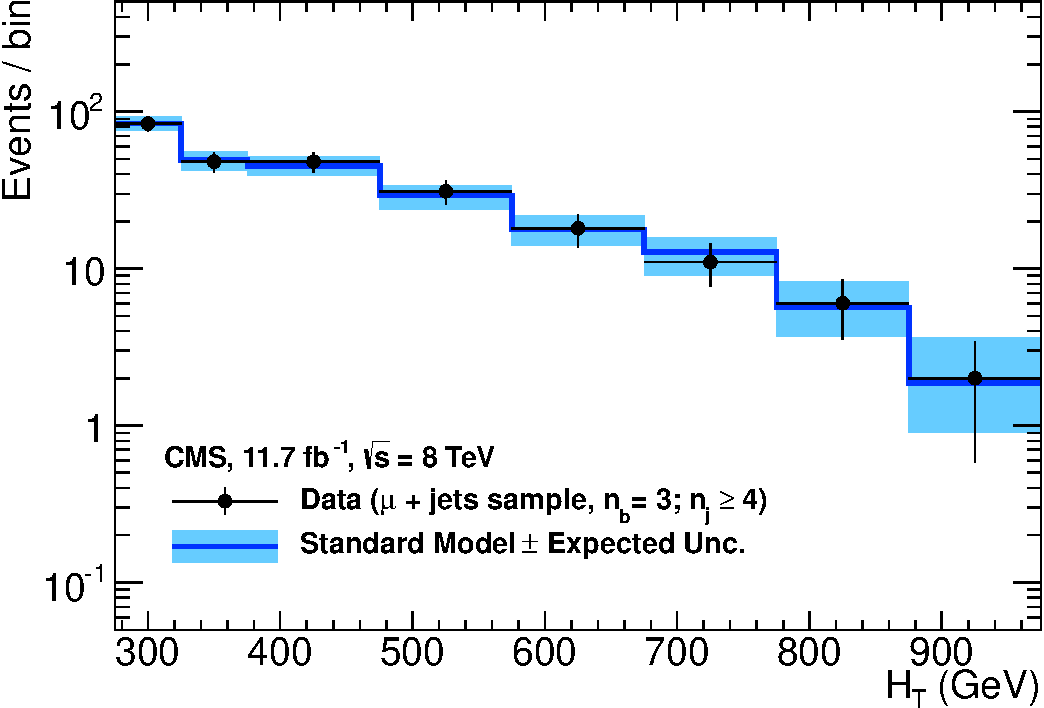
\includegraphics[width = 1.0\linewidth]{plots/muon_3b_ge4j_logy.pdf}
\centering (b)  \mupjets sample, $n_{jet} \geq 4$ and $n_{b}^{reco} = 3$  
\end{minipage} \\
\caption[Comparison of the observed yields and \ac{SM} expectations given by the simultaneous fit in bins of \theht for the (a) hadronic, (b) \mupjets, (c$)$ \dimupjets and (d) \gpjets samples when requiring $n_{b}^{reco}$ = 3 and $n_{jet} \geq 4$.]{Comparison of the observed yields and \ac{SM} expectations given by the simultaneous fit in bins of \theht for the (a) hadronic, (b) \mupjets, (c$)$ \dimupjets and (d) \gpjets samples when requiring $n_{b}^{reco}$ = 3 and $n_{jet} \geq 4$. The observed event yields in data (black dots) and the expectations and their uncertainties for all SM processes (blue line with light blue bands) are shown. An example signal expectation (red solid line) for the $G2$ \ac{SMS} signal point from Table \ref{tab:sms_model_table} is superimposed on the \ac{SM} background expectation.}
\label{fig:result3bhigh}
\end{figure}

\begin{figure}[ht]
\footnotesize
\centering
\begin{minipage}[b]{0.48 \linewidth}
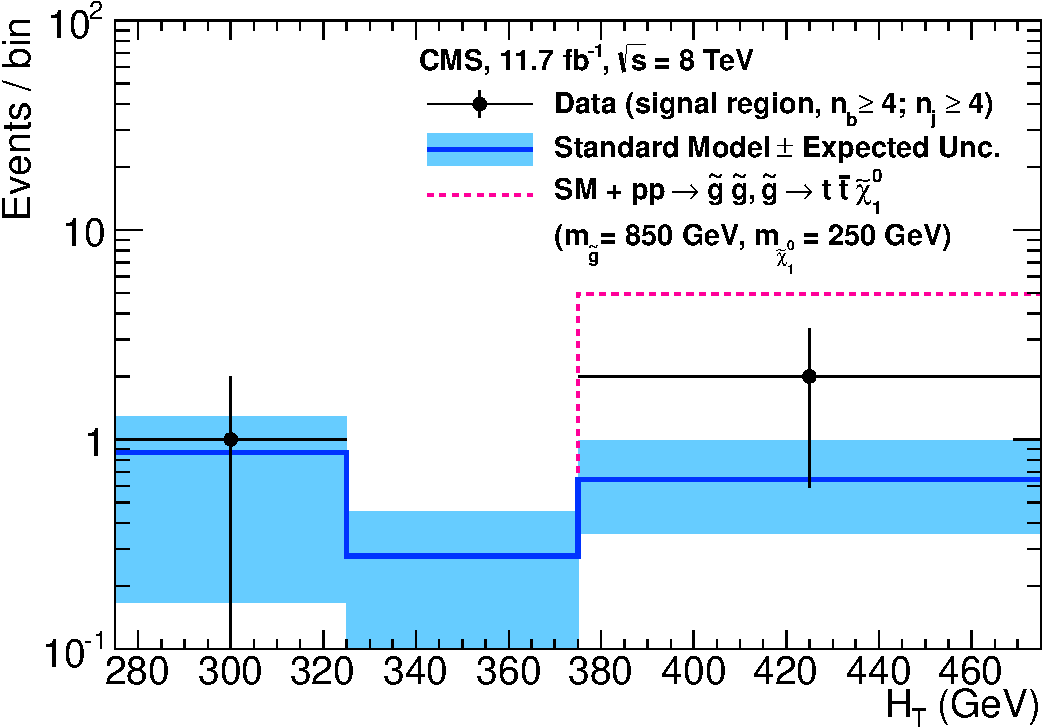
\includegraphics[width = 1.0\linewidth]{plots/hadronic_ge4b_ge4j_logy.pdf}
\centering (a)  Hadronic sample, $n_{jet} \geq 4$ and $n_{b}^{reco} \geq 4$ 
\end{minipage}
\quad
\begin{minipage}[b]{0.48\linewidth}
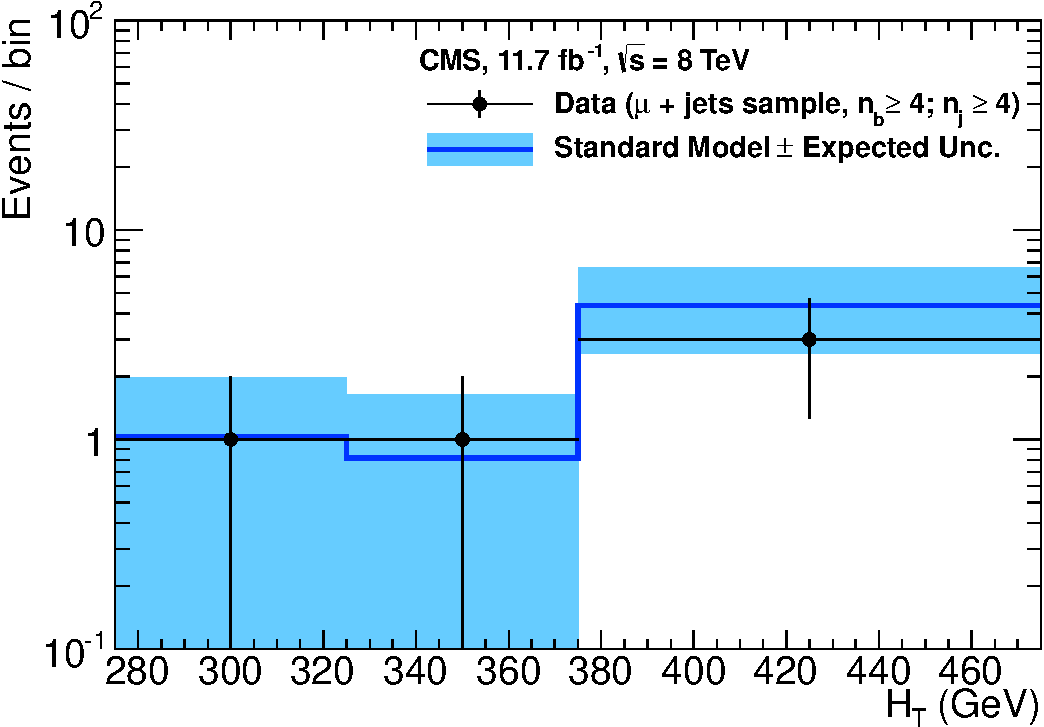
\includegraphics[width = 1.0\linewidth]{plots/muon_ge4b_ge4j_logy.pdf}
\centering (b)  \mupjets sample, $n_{jet} \geq 4$ and $n_{b}^{reco} \geq 4$  
\end{minipage} \\
\caption[Comparison of the observed yields and \ac{SM} expectations given by the simultaneous fit in bins of \theht for the (a) hadronic, (b) \mupjets, (c$)$ \dimupjets and (d) \gpjets samples when requiring $n_{b}^{reco} \geq$  4 and $n_{jet} \geq 4$.]{Comparison of the observed yields and \ac{SM} expectations given by the simultaneous fit in bins of \theht for the (a) hadronic, (b) \mupjets, (c$)$ \dimupjets and (d) \gpjets samples when requiring $n_{b}^{reco}$ $\geq$ 4 and $n_{jet} \geq 4$. The observed event yields in data (black dots) and the expectations and their uncertainties for all SM processes (blue line with light blue bands) are shown. An example signal expectation (red solid line) for the $G3$ \ac{SMS} signal point from Table \ref{tab:sms_model_table} is superimposed on the \ac{SM} background expectation.}
\label{fig:result4bhigh}
\end{figure}


\section{SUSY}
\label{sec:resultsms}

Limits are set in the parameter space of a set of \ac{SMS} models that characterise both natural \ac{SUSY} third generation squark production, and compressed spectra where the mass splitting between the particle and \ac{LSP} is small, leading to soft final state jets. However as detailed in Section (\ref{subsec:sms}), the individual models are not representative of a real physical \ac{SUSY} model as only one decay process is considered. Instead these models represent a way to test for signs of specific signatures indicating new physics. 

\subsection{The CL$_{\text{s}}$ Method}

The CLs method \cite{0954-3899-28-10-313}\cite{Junk1999435}\cite{Read:451614} is used to compute the limits for signal models, with the one-sided profile likelihood ratio as the test statistic \cite{asymptotictest}.

The test statistic is defined as
\begin{equation}
  q(\mu)=\begin{cases}
    -2\text{log}\lambda(\mu) & \text{ when $\mu \geq \hat{\mu}$},\\
      \ \ 0 & \text{otherwise}.
  \end{cases}
\end{equation}

where 

\begin{equation}
\lambda(\mu) = \frac{L(\mu,\theta_{\mu})}{L(\hat{\mu},\hat{\theta})}
\end{equation}

represents the profile likelihood ratio, in which $\mu \equiv f$ from Section (\ref{subsec:signalcontribution}), is the parameter characterising the signal strength.  $\hat{\mu}$ is defined as the maximum likelihood value, $\hat{\theta}$ the set of maximum likelihood values of the nuisance parameters and $\theta_{\mu}$ the set of maximum values of the nuisance parameters for a given value of $\mu$.

When $\mu \equiv f = 1$, the signal model is considered at its nominal production cross section. The distribution of $q_{\mu}$ is built up via the generation of pseudo experiments in order to obtain two distributions for the background (B) and signal plus background (S+B) cases.

The compatibility of a signal model with observations in data is determined by the parameter CL$_{s}$,

\begin{equation}
\text{CL$_{S}$} = \frac{\text{CL$_{S+B}$}}{\text{CL$_{B}$}},
\end{equation}

with CL$_{B}$ and CL$_{S+B}$ defined as one minus the quantiles of the observed value in the data of the two distributions. A model is considered to be excluded at 95\% confidence level when CL$_{s} \leq 0.05$ \cite{2011EPJClimits}.

\subsection{Interpretation in Simplified Signal Models}

Different \njet and \nbreco bins are used in the interpretation of different \ac{SMS} models. The choice of categories used, are made such that the signal to background ratio will be maximised for the model in question, increasing sensitivity to that particular type of final state signature. The production and decay modes of the \ac{SMS} models under consideration are summarised in Table \ref{tab:susyresults}, with limit plots of the experimental reach in these models shown in Figure \ref{fig:smslimitplots}.

The models \texttt{T1} and \texttt{T2} are used to characterise the pair production of gluinos and first or second generation squarks respectively. The low number of third generation quarks produced from this decay topology makes choosing to interpret within the \nbreco = 0 category beneficial to improving sensitivity to these models. In the case of the \texttt{T2} model, two sets of exclusion contours are shown. These correspond to the production of eight first- and second-generation (left-/right-handed) squarks with degenerate masses and the case of just a single light squark with all other squarks decoupled at much higher masses.

Conversely the \texttt{T2bb}, \texttt{T1tttt}, and \texttt{T1bbbb} \ac{SMS} models describe various production and decay mechanisms in the context of third-generation squarks. In this situation considering higher \nbreco categories bring significant improvements to the sensitivity to these types of final state signature. 

Finally the choice of jet category is made dependant upon the production mechanism, where gluino induced and direct squark production results in a large or small number of final state jets respectively.

 \begin{table}[h!]
 \footnotesize
\begin{center}
\begin{tabular*}{1.0\textwidth}{@{\extracolsep{\fill}}llcccccc}
\hline
Model & Production/decay & $n_{jet}$ & $n_{b}^{reco}$ & Process & Limit & m$_{\tilde{q}(\tilde{g})}^{\text{best}}$ (\GeV)  & m$_{\text{LSP}}^{\text{best}}$ (\GeV) \\
\hline\hline
\texttt{T1} &  $pp \rightarrow \widetilde{g}\widetilde{g}^{*} \rightarrow q\bar{q}\widetilde{\chi}^{0}_{1}q\bar{q}\widetilde{\chi}^{0}_{1}$ & $\geq 4$ & 0 & \ref{fig:smsprocesses}(a) & \ref{fig:smslimitplots}(a) & $\sim$950 & $\sim$450 \\
\texttt{T2}  & $ pp \rightarrow \widetilde{q}\widetilde{q}^{*} \rightarrow q\widetilde{\chi}^{0}_{1}\bar{q}\widetilde{\chi}^{0}_{1}$ & $\leq 3$ & 0 & \ref{fig:smsprocesses}(b) & \ref{fig:smslimitplots}(b) & $\sim$775 &  $\sim$325 \\
\texttt{T2bb} & $ pp \rightarrow \widetilde{b}\widetilde{b}^{*} \rightarrow b\widetilde{\chi}^{0}_{1}\bar{b}\widetilde{\chi}^{0}_{1}$ & $\leq 3$ & 1,2 & \ref{fig:smsprocesses}(c$)$ & \ref{fig:smslimitplots}(c$)$ & $\sim$600 & $\sim$200\\
\texttt{T1tttt} & $ pp \rightarrow \widetilde{g}\widetilde{g}^{*} \rightarrow t\bar{t}\widetilde{\chi}^{0}_{1}t\bar{t}\widetilde{\chi}^{0}_{1}$ & $\geq 4$ & 2,3,$\geq4$ & \ref{fig:smsprocesses}(d) & \ref{fig:smslimitplots}(d) & $\sim$975 & $\sim$325 \\
\texttt{T1bbbb} & $ pp \rightarrow \widetilde{g}\widetilde{g}^{*} \rightarrow b\bar{b}\widetilde{\chi}^{0}_{1}b\bar{b}\widetilde{\chi}^{0}_{1}$ & $\geq 4$ & 2,3,$\geq4$ & \ref{fig:smsprocesses}(e) & \ref{fig:smslimitplots}(e) & $\sim$1125 & $\sim$650 \\
\hline
\end{tabular*}
\end{center}
\caption[A table representing the \ac{SMS} models interpreted within the analysis.]{A table representing the \ac{SMS} models interpreted within the analysis. The model name and production and decay chain is specified in the first two columns. Each \ac{SMS} model is interpreted in specific $n_{jet}$ and $n_{b}^{reco}$ categories which are detailed in the third and fourth columns. The last two columns indicate the search sensitivity for each model, representing the largest $m_{\widetilde{q}/\widetilde{g}}$ mass beyond which no limit can be set for this particular decay topology. The quoted values are conservatively determined from the observed exclusion based on the theoretical production cross section minus 1$\sigma$ uncertainty.}\label{tab:susyresults}
\end{table}


Experimental uncertainties on the \ac{SM} background predictions (10 $-$ 30\%, described in Section (\ref{subsec:determinesystematics})), the luminosity measurement (4.4\%), and the total acceptance times efficiency of the selection for the considered signal model (12 $-$18\%, from Section (\ref{sec:smsmodels})) are included in the calculation of the limit. 

Signal efficiency in the kinematic region defined by 0 $< m_{\widetilde{g}(\widetilde{q})} <$ 175 \GeV or $m_{\widetilde{g}(\widetilde{q})} <$ 300 \GeV is strongly affected by the presence of \acf{ISR}. This is a region in which direct (i.e. non-\ac{ISR} induced) production is kinematically forbidden due to the \theht $>$ 275 \GeV requirement, therefore a large percentage of signal acceptance is due to the effect of \ac{ISR} jets. Given the large associated uncertainties, no interpretation is provided for this kinematic region.

The estimates on mass limits shown in Table  \ref{tab:susyresults}, are determined conservatively from the observed exclusion based on the theoretical production cross section, minus 1$\sigma$ uncertainty. The most stringent mass limits on pair-produced sparticles are obtained at low \ac{LSP} masses and larger squark and gluino masses due to the high \pt jets and consequently high \theht of such signal topologies. The limits are seen to weaken for compressed spectra points closer to the diagonal, where the signal populates the lower \theht bins in which more background resides. For all of the considered models, there is an \ac{LSP} mass beyond which no limit can be set, which can be observed from the figures referenced in the table. 

Two small upwards fluctuations are observed within the data, and are seen at high \theht within the \nbreco = 0 category and at mid-\theht in the \nbreco = 1, 2 categories, see Table \ref{tab:fitsdata}. As each of these fluctuations occur within at least one of the analysis categories that each \ac{SMS} model interpretation is made, the observed exclusions within all \ac{SMS} models are generally found to be weaker than the expected limits in the region of 1-2 standard deviations. In isolation these fluctuations are not significant and additional data would be necessary to make any further conclusions.

Despite these fluctuations, the range of parameter space that can be excluded has been extended with respect to analysis based upon the $\sqrt{s} = 7$ \TeV dataset \cite{Chatrchyan:2012wa}, by up to 225 and 150 \GeV for m$_{\tilde{q}(\tilde{g})}^{\text{best}}$ and m$_{LSP}^{\text{best}}$ respectively. The parameter space for light third generation squarks, the main tenet of natural \ac{SUSY} models, is increasingly squeezed for larger mass splitting, with exclusions in the region of 1 \TeV in these topologies. 



\begin{figure}[ht]
\footnotesize
\centering
\begin{minipage}[b]{0.48 \linewidth}
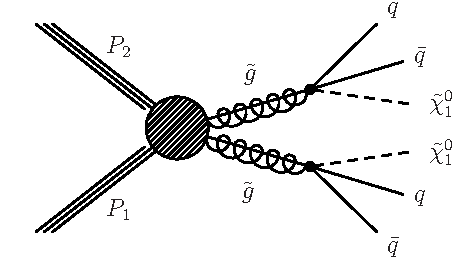
\includegraphics[width = 1.0\linewidth]{plots/t1susydecay.pdf}
\centering \caption*{(a) $\widetilde{g}\widetilde{g}^{*} \rightarrow q\bar{q}\widetilde{\chi}^{0}_{1}q\bar{q}\widetilde{\chi}^{0}_{1}$ (\texttt{T1})}\label{f`ig:t1}
\end{minipage}
\quad
\begin{minipage}[b]{0.48\linewidth}
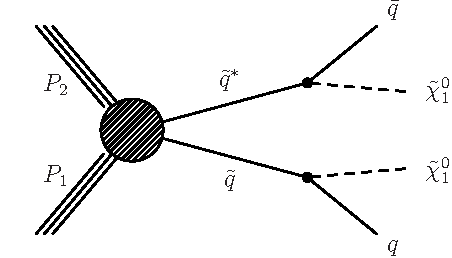
\includegraphics[width = 1.0\linewidth]{plots/t2susydecay.pdf}
\centering \caption*{(b) $\widetilde{q}\widetilde{q}^{*} \rightarrow q\widetilde{\chi}^{0}_{1}\bar{q}\widetilde{\chi}^{0}_{1}$ (\texttt{T2})} \label{fig:t2}
\end{minipage} \\
\vspace{0.4cm}
\begin{minipage}[b]{0.48 \linewidth}
\includegraphics[width = 1.0\linewidth]{plots/t2bbsusydecay.pdf}
\centering \caption*{(c$)$ $\widetilde{b}\widetilde{b}^{*} \rightarrow b\widetilde{\chi}^{0}_{1}\bar{b}\widetilde{\chi}^{0}_{1}$ (\texttt{T2bb})} \label{fig:t2bb}
\end{minipage}
\quad
\begin{minipage}[b]{0.48\linewidth}
\includegraphics[width = 1.0\linewidth]{plots/t1ttttsusydecay.pdf}
\centering \caption*{(d) $\widetilde{g}\widetilde{g}^{*} \rightarrow t\bar{t}\widetilde{\chi}^{0}_{1}t\bar{t}\widetilde{\chi}^{0}_{1}$ (\texttt{T1tttt})} \label{fig:t2tttt}
\end{minipage}
\quad
\begin{minipage}[b]{0.48\linewidth}
\centering
\includegraphics[width = 1.0\linewidth]{plots/t1bbbbsusydecay.pdf}
\centering \caption*{(e) $\widetilde{g}\widetilde{g}^{*} \rightarrow b\bar{b}\widetilde{\chi}^{0}_{1}b\bar{b}\widetilde{\chi}^{0}_{1}$ (\texttt{T1bbbb})} \label{fig:t1bbbb}
\end{minipage}
\caption[Production and decay modes for the various \ac{SMS} models interpreted within the analysis.]{Production and decay modes for the various \ac{SMS} models interpreted within the analysis.}
\label{fig:smsprocesses}
\end{figure}

\begin{figure}[ht]
\footnotesize
\centering
\begin{minipage}[b]{0.48 \linewidth}
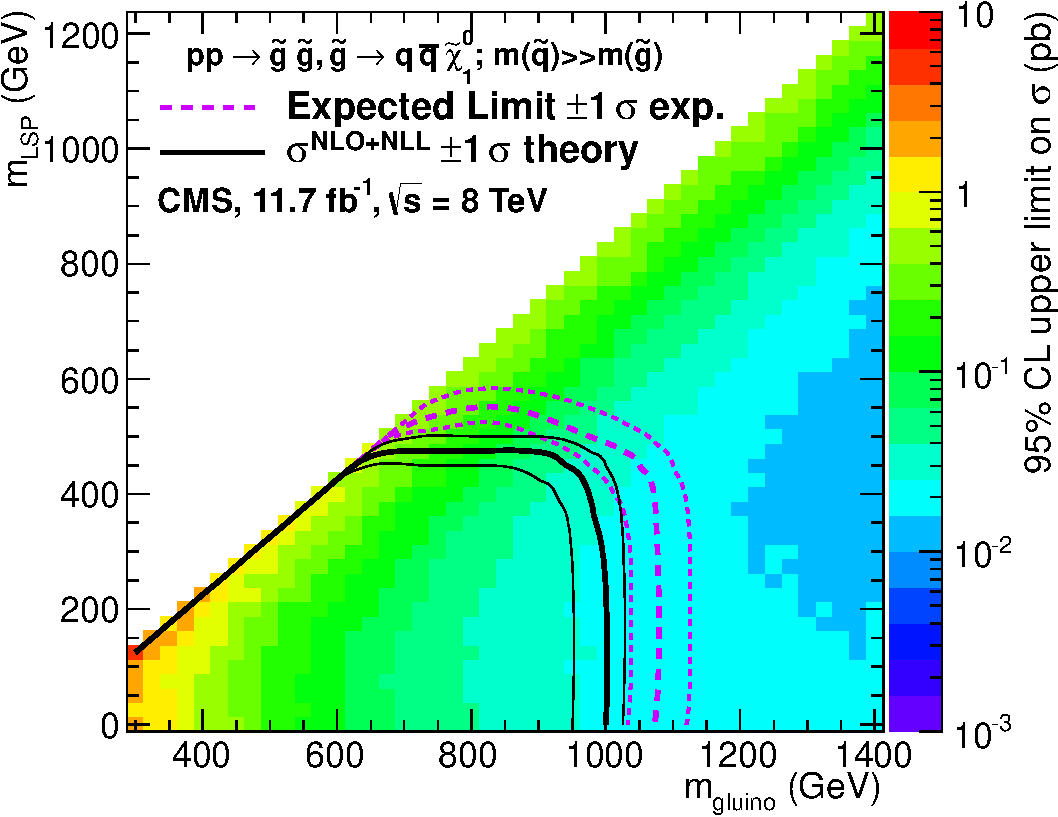
\includegraphics[width = 1.0\linewidth]{plots/t1.pdf}
\centering \caption*{(a) $\widetilde{g}\widetilde{g}^{*} \rightarrow q\bar{q}\widetilde{\chi}^{0}_{1}q\bar{q}\widetilde{\chi}^{0}_{1}$ (\texttt{T1})}\label{fig:t1}
\end{minipage}
\quad
\begin{minipage}[b]{0.48\linewidth}
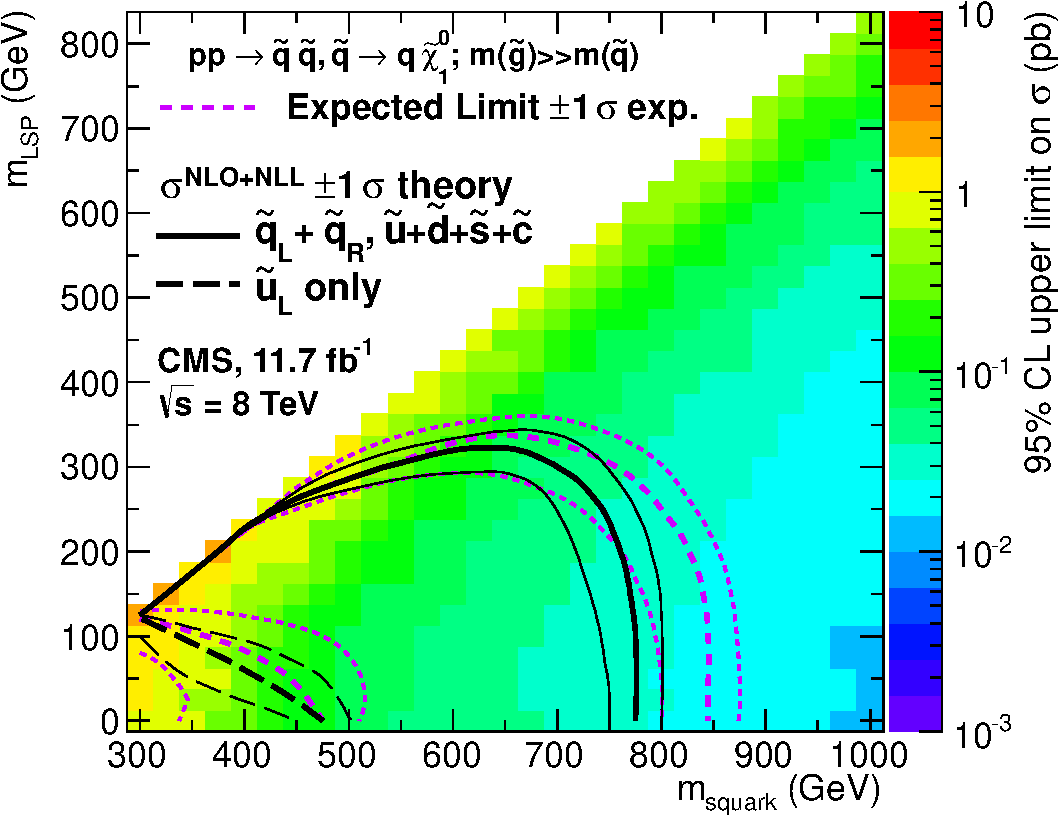
\includegraphics[width = 1.0\linewidth]{plots/t2.pdf}
\centering \caption*{(b) $\widetilde{q}\widetilde{q}^{*} \rightarrow q\widetilde{\chi}^{0}_{1}\bar{q}\widetilde{\chi}^{0}_{1}$ (\texttt{T2})} \label{fig:t2}
\end{minipage} \\
\vspace{0.4cm}
\begin{minipage}[b]{0.48 \linewidth}
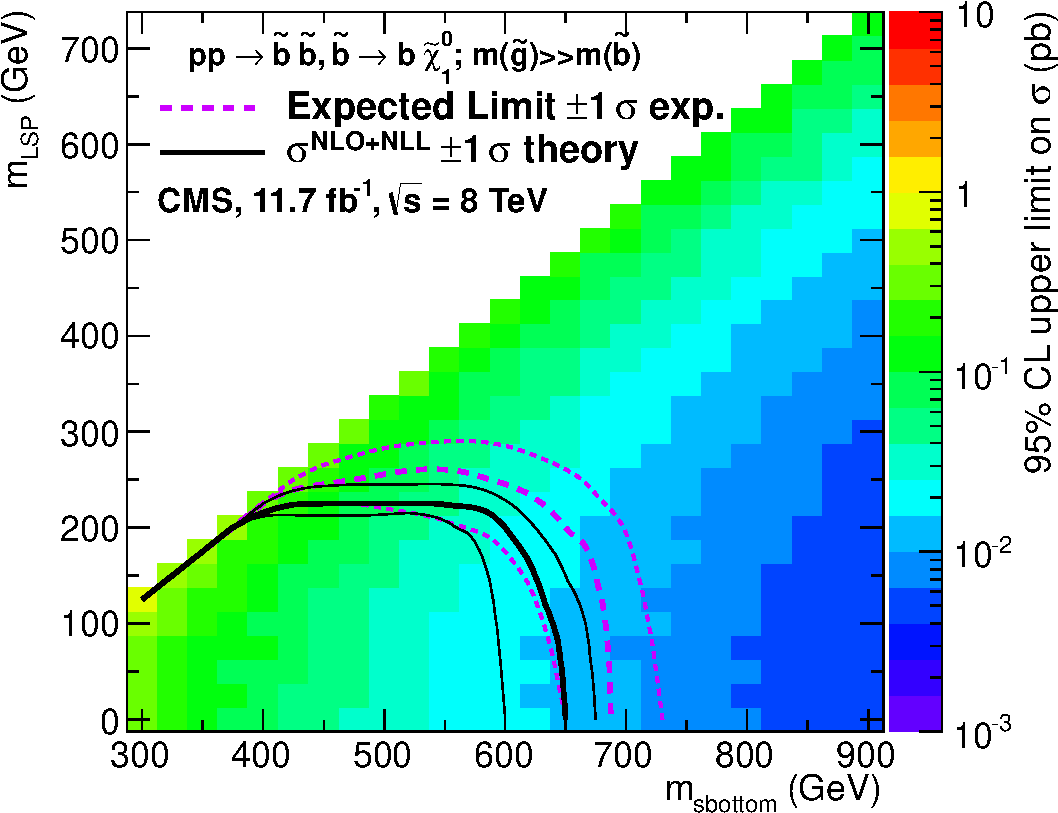
\includegraphics[width = 1.0\linewidth]{plots/t2bb.pdf}
\centering \caption*{(c$)$ $\widetilde{b}\widetilde{b}^{*} \rightarrow b\widetilde{\chi}^{0}_{1}\bar{b}\widetilde{\chi}^{0}_{1}$ (\texttt{T2bb})} \label{fig:t2bb}
\end{minipage}
\quad
\begin{minipage}[b]{0.48\linewidth}
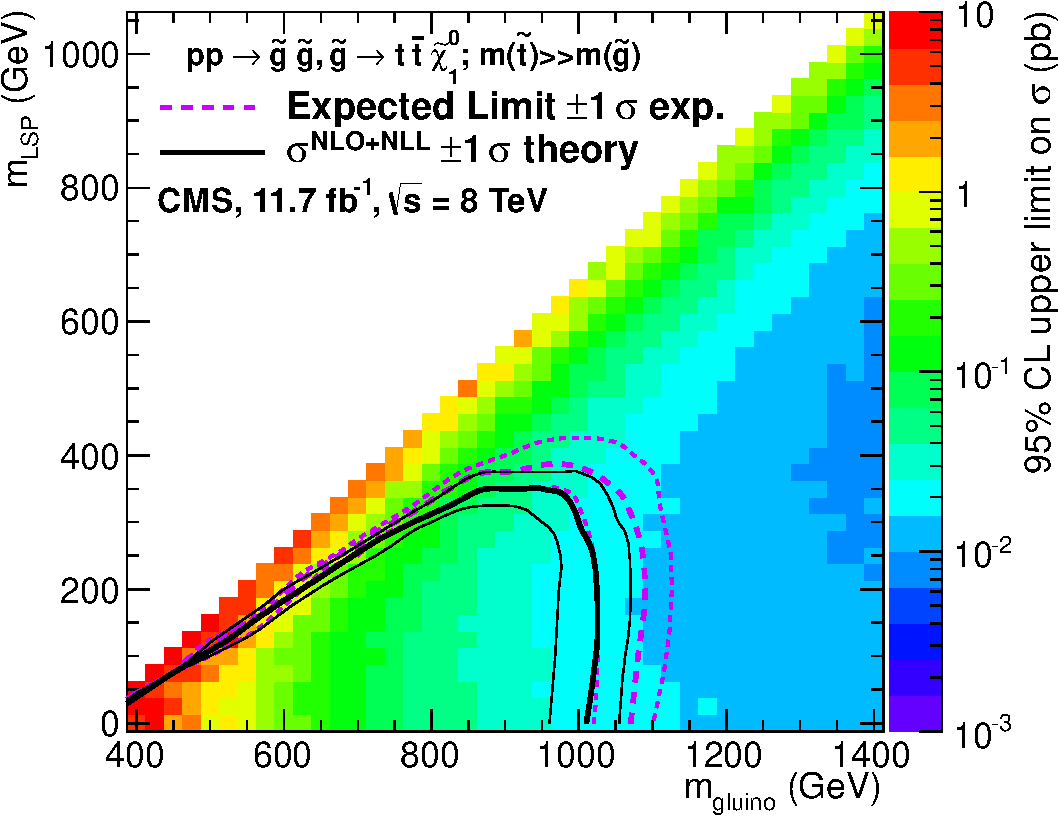
\includegraphics[width = 1.0\linewidth]{plots/t1tttt.pdf}
\centering \caption*{(d) $\widetilde{g}\widetilde{g}^{*} \rightarrow t\bar{t}\widetilde{\chi}^{0}_{1}t\bar{t}\widetilde{\chi}^{0}_{1}$ (\texttt{T1tttt})} \label{fig:t2tttt}
\end{minipage}
\quad
\begin{minipage}[b]{0.48\linewidth}
\centering
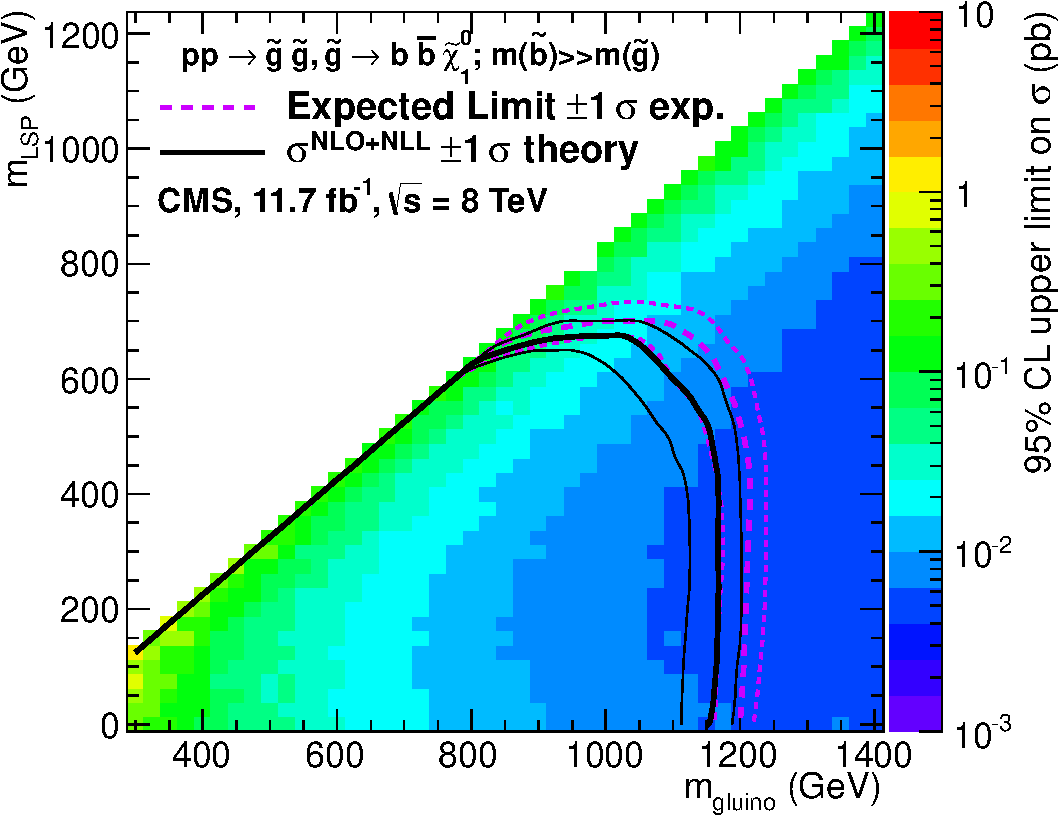
\includegraphics[width = 1.0\linewidth]{plots/t1bbbb.pdf}
\centering \caption*{(e) $\widetilde{g}\widetilde{g}^{*} \rightarrow b\bar{b}\widetilde{\chi}^{0}_{1}b\bar{b}\widetilde{\chi}^{0}_{1}$ (\texttt{T1bbbb})} \label{fig:t1bbbb}
\end{minipage}
\caption[Upper limit of cross section at 95\% CL as a function of $m_{\widetilde{q}/\widetilde{g}}$ and $m_{LSP}$ for various \ac{SMS} models.]{Upper limit of cross section at 95\% CL as a function of $m_{\widetilde{q}/\widetilde{g}}$ and $m_{LSP}$ for various \ac{SMS} models. The solid thick black line indicates the observed exclusion region assuming \ac{NLO} and \ac{NLL}  SUSY production cross section. The analysis selection efficiency is measured for each interpreted model, with the signal yield per point given by $\epsilon \times \sigma$. The thin black lines represent the observed excluded region when varying the cross section by its theoretical uncertainty. The dashed purple lines indicate the median (thick line) �1$\sigma$ (thin lines) expected exclusion regions.}
\label{fig:smslimitplots}
\end{figure}



